% vim: set tw=78 tabstop=8 shiftwidth=2 softtabstop=2 aw ai:
\documentclass{beamer}

\usepackage[utf8x]{inputenc}            % diacritice
\usepackage[english]{babel}
\usepackage{color}                      % highlight
\usepackage{alltt}                      % highlight
%\usepackage{code/highlight}            % highlight
\usepackage{hyperref}                   % folosiți \url{http://...}
                                        % sau \href{http://...}{Nume Link}
\usepackage{verbatim}
\usepackage{subfigure}
\usepackage{booktabs}

% Show contents at every section beginning. Ripped off from manual.
\AtBeginSection[] % Do nothing for \section*
{
  \begin{frame}<beamer>
    \frametitle{Outline}
  \tableofcontents[currentsection]
    \end{frame}
}

\mode<presentation>
{ \usetheme{Berlin} }

% Încărcăm simbolurilor Unicode românești în titlu și primele pagini
\PrerenderUnicode{aâîțșĂÎÂȚȘ}

\title[Protocol Measurements and Improvements in Peer-to-Peer
Systems]{Protocol Measurements and Improvements in Peer-to-Peer Systems}
\subtitle{PhD Thesis}
\institute[CSE, ACS, UPB]{University POLITEHNICA of Bucharest}
\author[Răzvan Deaconescu]{Author: drd. Răzvan Deaconescu\\
Supervisor: prof. dr. ing. Nicolae Țăpuș}
\date{September 28, 2011}

\begin{document}

% Slide-urile cu mai multe părți sunt marcate cu textul (cont.)
\setbeamertemplate{frametitle continuation}[from second]

% Arătăm numărul frame-ului
% \setbeamertemplate{footline}[frame number]

\frame{\titlepage}

\section{Introduction}

\begin{frame}{Objective}
  \begin{itemize}
    \item providing a series of improvements to Peer-to-Peer systems at
    protocol level, either through updating and enhancing existing protocols
    or designing and implementing new ones
    \item formal and experimental evaluations -- arguments regarding the
    advantages of updates
    \item careful trial deployment and analysis of Peer-to-Peer protocols
    \item methods and mechanisms for creating realistic, scalable and
    automated trial environments
    \item the approaches available for collecting, measuring and interpreting
    Peer-to-Peer protocol parameters
  \end{itemize}
\end{frame}

\begin{frame}{Scope}
  \begin{itemize}
    \item Peer-to-Peer
    \item BitTorrent
    \item client-centric
    \item protocol parameters (low-level information)
    \item protocool improvements
  \end{itemize}
\end{frame}

\begin{frame}{Context}
  \begin{itemize}
    \item EU FP7 P2P-Next
    \item BitTorrent
    \item swift
    \item streaming
    \item LivingLab
    \item P2P streaming
    \item virtualization
    \item client-based logging
  \end{itemize}
\end{frame}

\section{Peer-to-Peer Systems}

\begin{frame}{Peer-to-Peer}
  \begin{figure}
    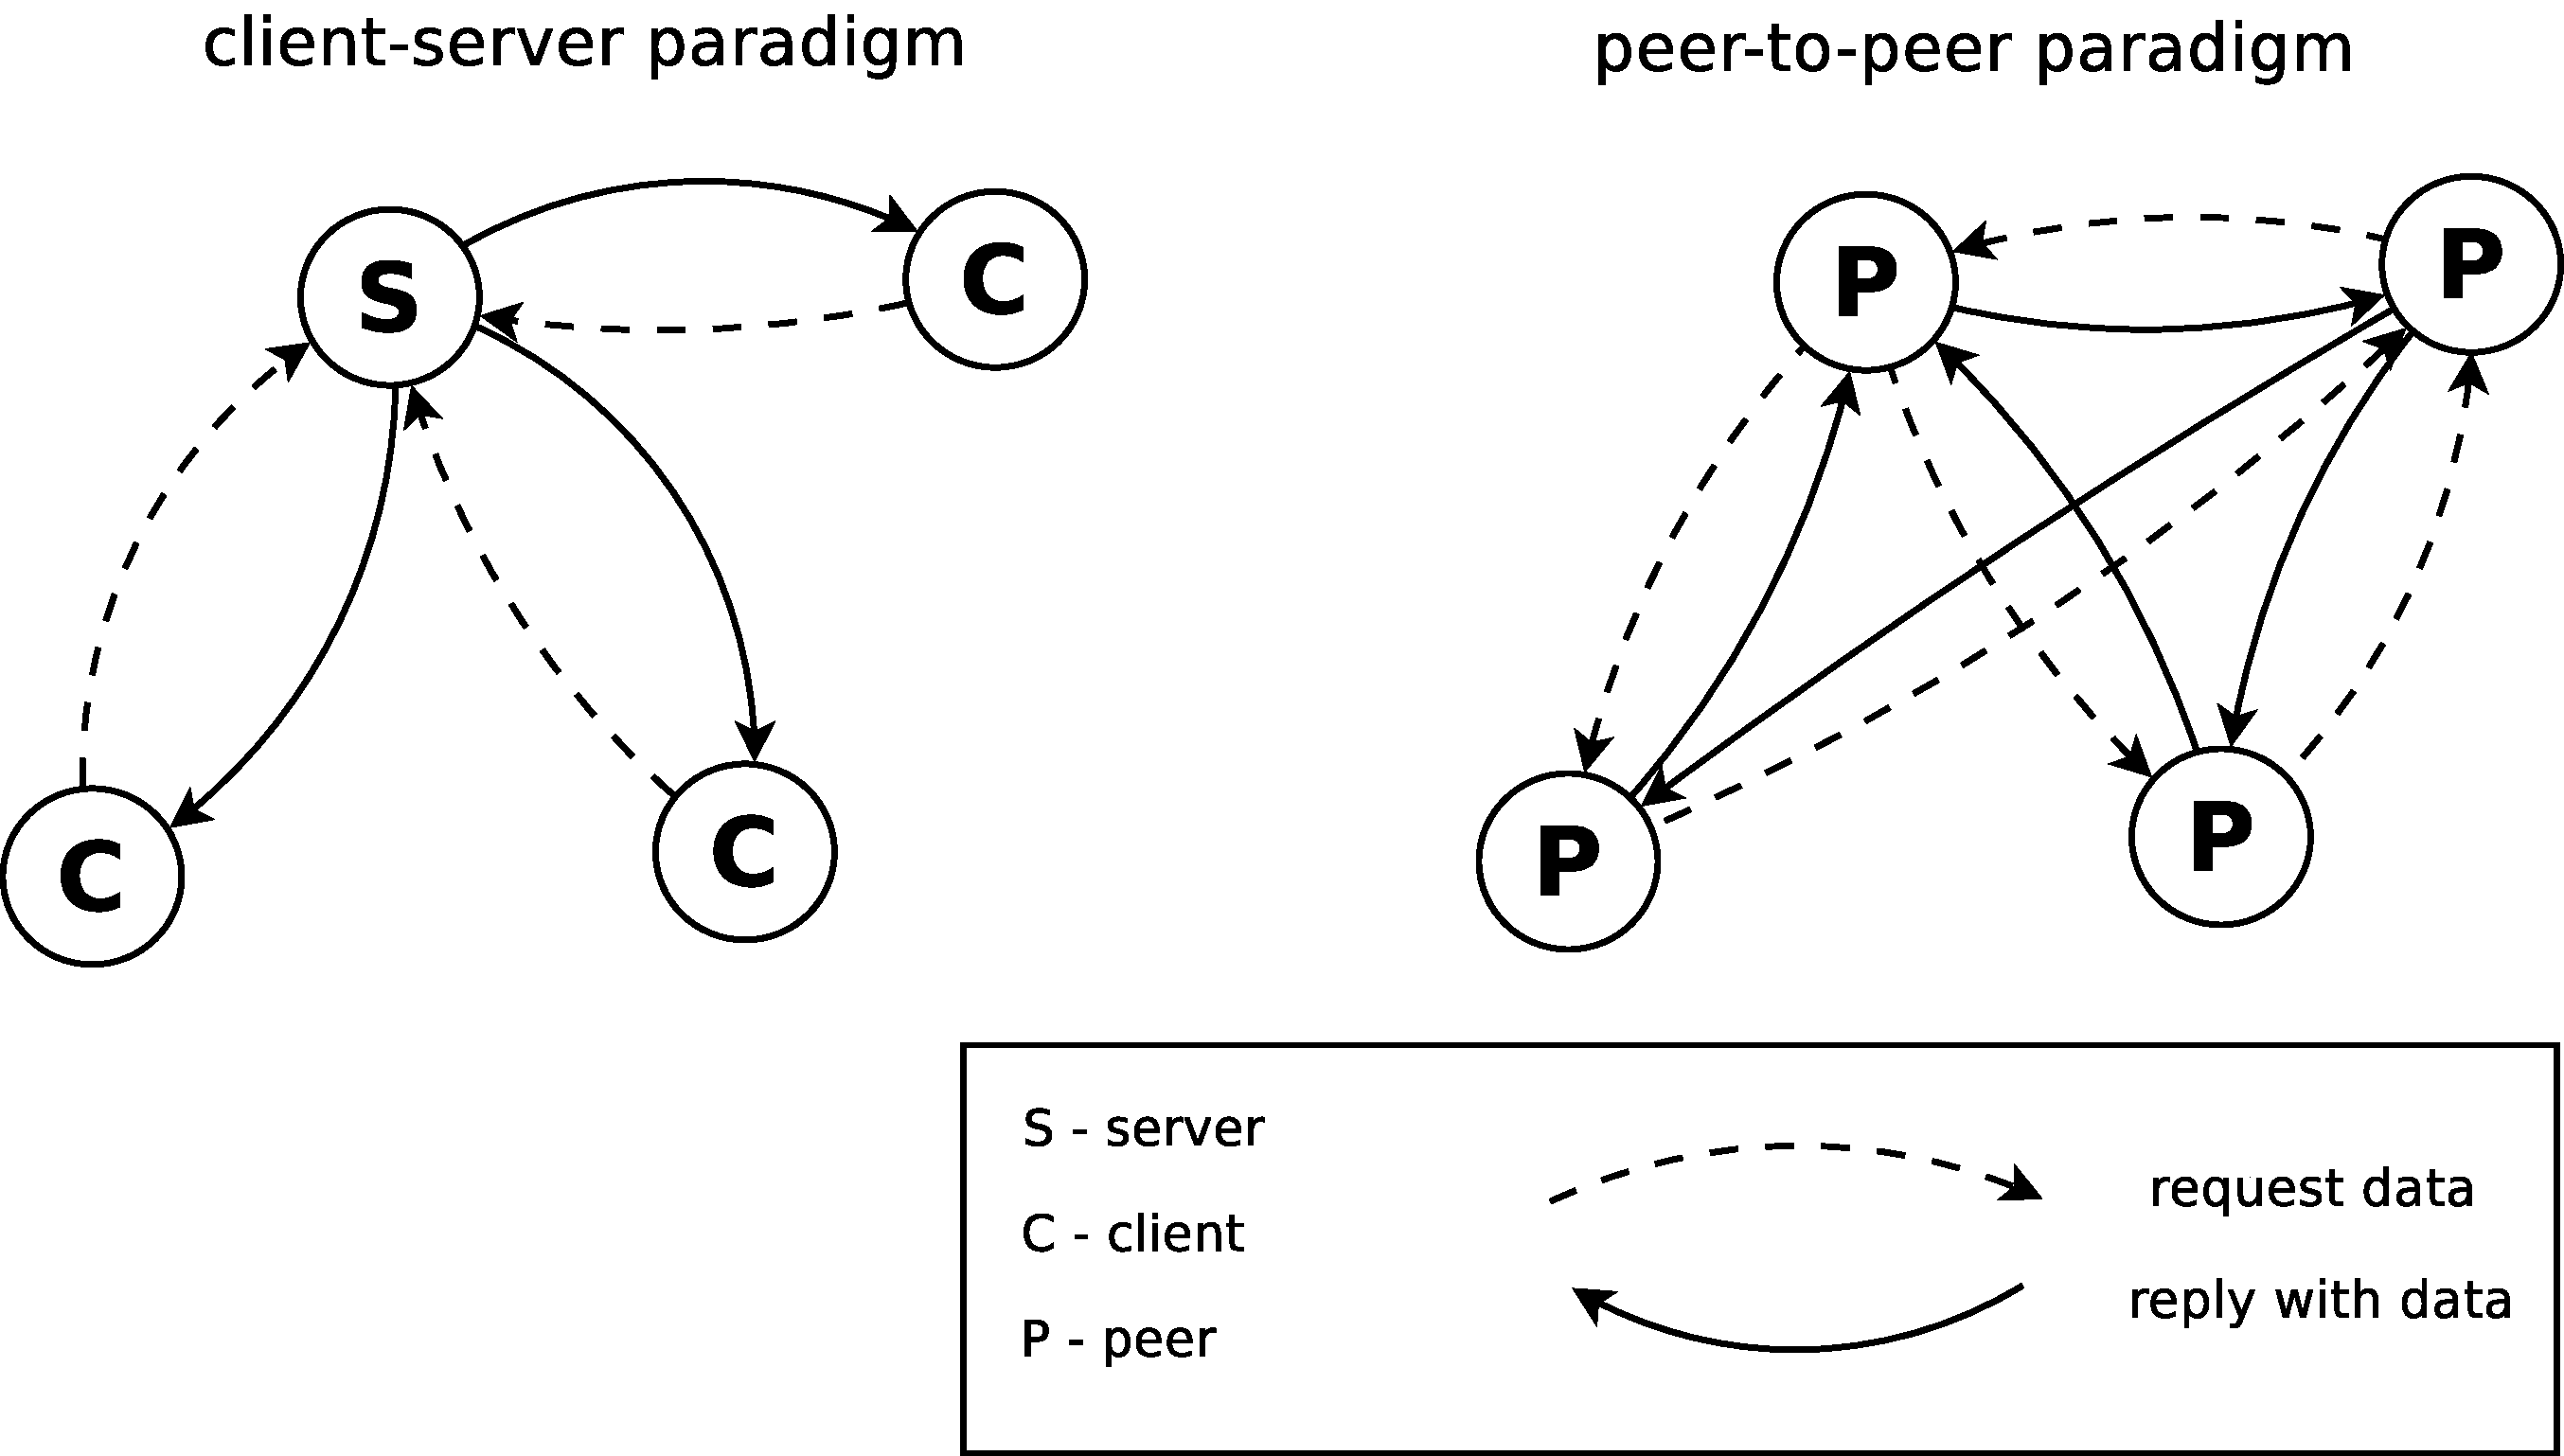
\includegraphics[width=0.9\textwidth]{img/client-server-vs-p2p}
  \end{figure}
\end{frame}

\begin{frame}{BitTorrent}
  \begin{figure}
    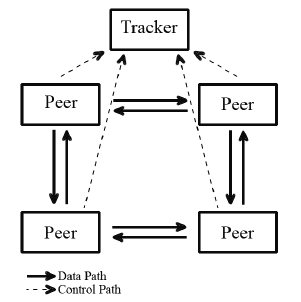
\includegraphics[width=0.6\textwidth]{img/bittorrent-overview}
  \end{figure}
\end{frame}

\begin{frame}{Content Distribution}
  \begin{itemize}
    \item producer, consumer, \textbf{prosumer}
    \item video source, video client
    \item download protocol, video playback
    \item offline playback
    \item Video-on-Demand (VoD)
    \item Live Streaming
    \item Content Delivery Networks (CDNs)
  \end{itemize}
\end{frame}

\begin{frame}{Streaming in Peer-to-Peer}
  \begin{itemize}
    \item a peer is the video source
    \item other peers are clients and relay agents
    \item multiple distribution paths
    \item the need of a P2P network overlay over the physical network
  \end{itemize}
\end{frame}

\section{Infrastructure}

\begin{frame}{Measurements in Peer-to-Peer Systems}
  \begin{itemize}
    \item testbeds (PlanetLab)
    \item simulations
    \item real world scenarios
      \begin{itemize}
        \item data collection and storage
        \item trackers
      \end{itemize}
  \end{itemize}
\end{frame}

\begin{frame}{Virtualization}
  \begin{itemize}
    \item hardware/server virtualization
    \item multiple instances of separate OSs running on same hardware
    \item hypervisor (VMM)
    \item consolidation, reliability, security
    \item full virtualization, paravirtualization, OS-level virtualization
  \end{itemize}
\end{frame}

\begin{frame}{Goals}
  \begin{itemize}
    \item automated infrastructure for BitTorrent clients
    \item scalable and flexible (virtualization)
    \item complete control over swarm environment (private infrastructure)
    \item intensive client information (client logging)
    \item performance evaluation and comparison
    \item internal protocol analysis
  \end{itemize}
\end{frame}

\begin{frame}{OpenVZ}
  \begin{itemize}
    \item OS-level virtualization
    \item low overhead (extended chroot) -- runs directly on top of operating
    system
    \item templates
    \item CLI-interaction (\texttt{vzctl}) -- automation
    \item resource limitation (user beancounters)
  \end{itemize}
\end{frame}

\begin{frame}{Overall View}
  \begin{figure}
    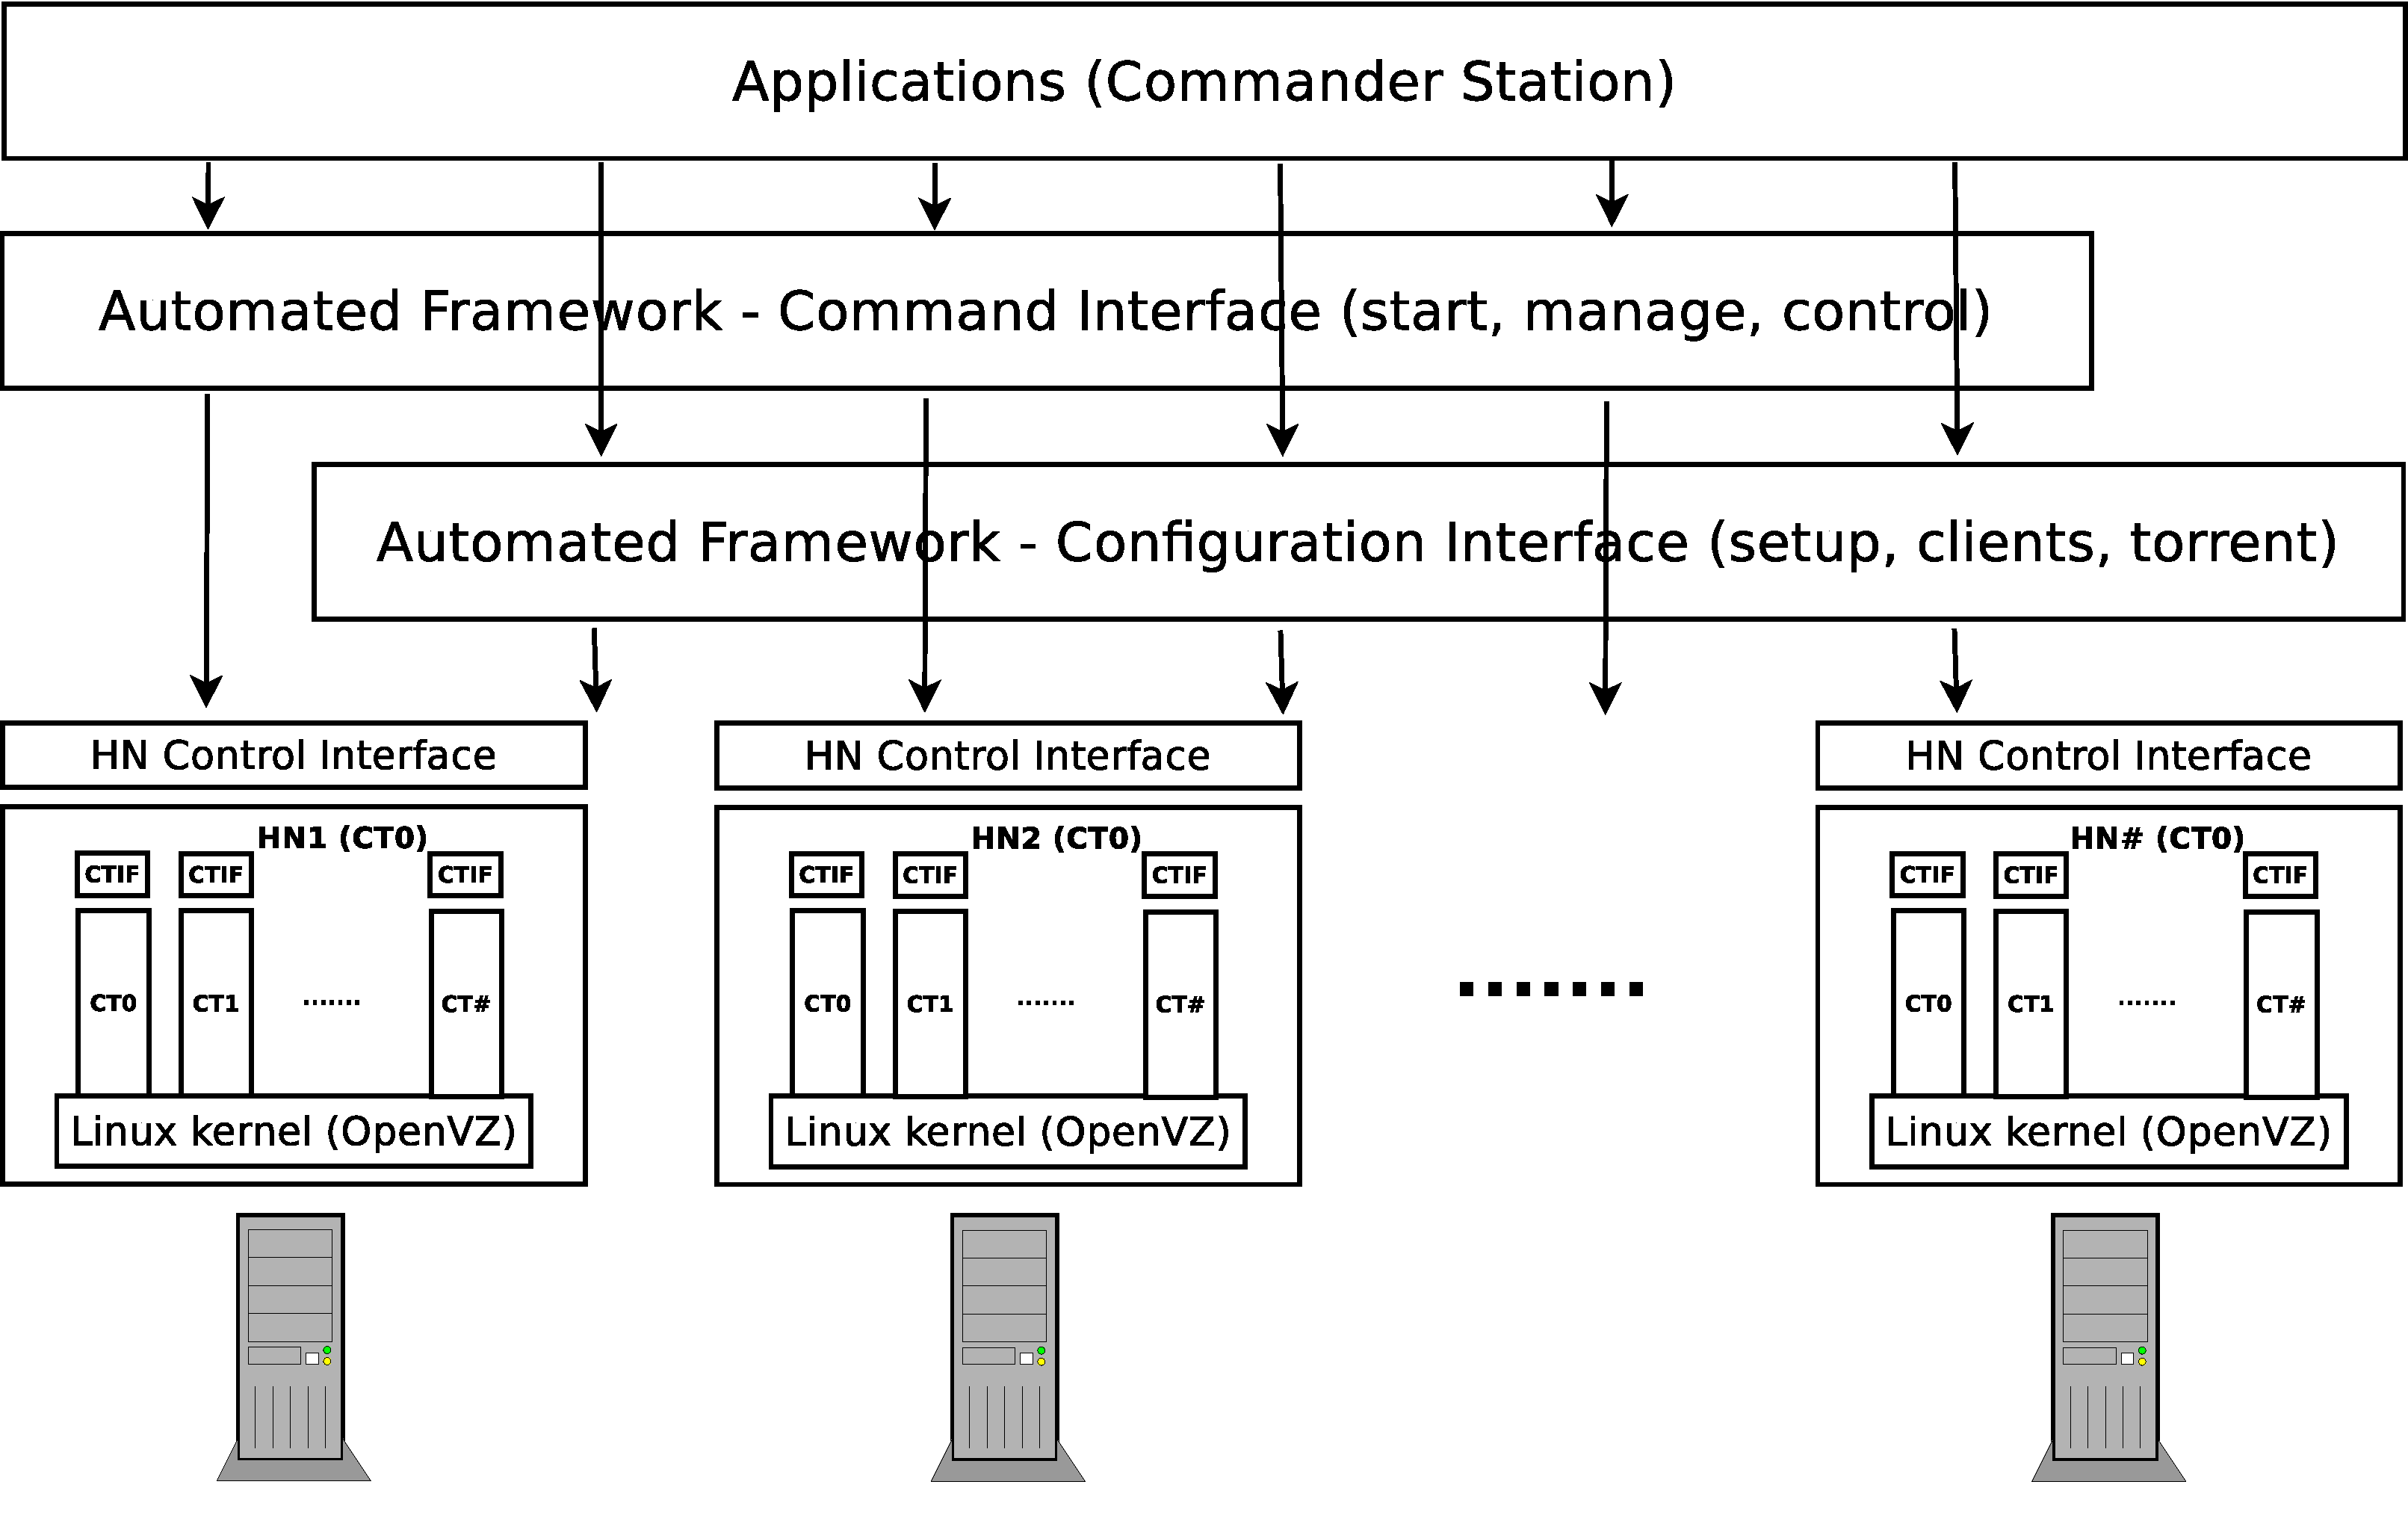
\includegraphics[scale=0.17]{img/virt-infra-overview}
  \end{figure}
\end{frame}

\begin{frame}{Tools Employed}
  \begin{itemize}
    \item vzctl + templates
    \item shell scripting
    \item SSH
    \item tc (traffic control)
    \item iptables
    \item brctl
    \item sysstat
  \end{itemize}
\end{frame}

\begin{frame}{Virtualization Evaluation}
  \begin{itemize}
    \item \textbf{efficiency} (scalability) -- how many virtual
    machines/containers may be deployed on a virtual host and allow proper
    simulation of an environment;
    \item \textbf{isolation} -- how well are virtual machines' resources
    separated;
    \item \textbf{reliability} -- how many software crashes happen for a given
    solution; this may be due to implementation or to resourse overuse/abuse.
  \end{itemize}
\end{frame}

\begin{frame}{Virtualization Evaluation (2)}
  \scriptsize
  \begin{align}
    Eff &= f(HW, SW, VS)\\
    Eff &= f(RAM, HDD, CPU, NET, OS, PS, BT, VS, NVM)\\
    Eff &= \frac{VMB}{HNB}
  \end{align}
  \begin{align}
    Iso(normal processes) < Iso(chroot) < Iso(OpenVZ, LXC) < Iso(Xen,KVM)
  \end{align}
  \begin{align}
    Rel &= f(HW, SW, VS)\\
    Rel &= f(RAM, HDD, CPU, OS (filesystem), PS, BT, VS, NVM)
  \end{align}
\end{frame}

\section{Automated Framework}

\begin{frame}{Architecture}
  \begin{figure}
    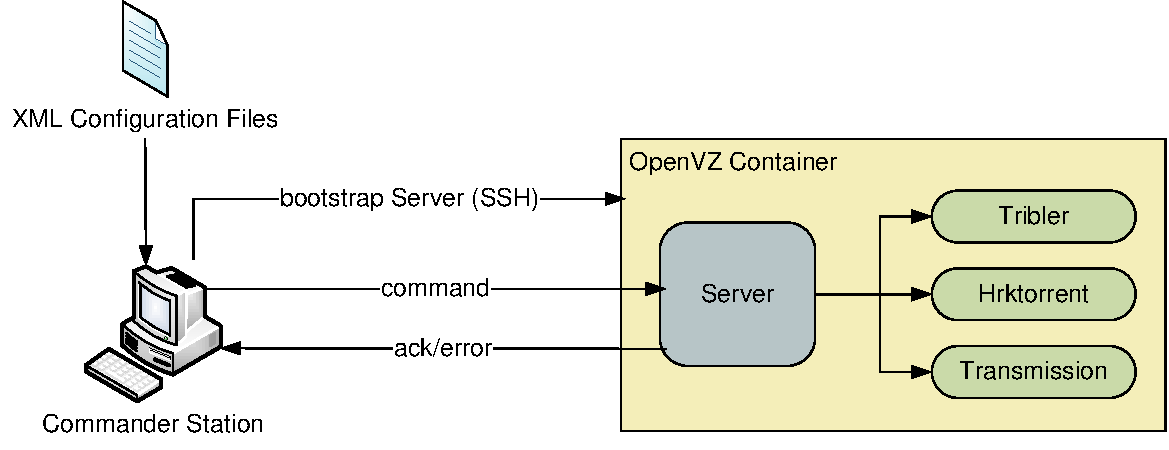
\includegraphics[scale=0.5]{img/service-arch}
  \end{figure}
\end{frame}

\begin{frame}{Goals}
  \begin{itemize}
    \item automation
    \item complete control (internal swarms vs. external swarms)
    \item full client information
  \end{itemize}
\end{frame}

\begin{frame}{Client Instrumentation}
  \begin{itemize}
    \item open-source clients
    \item update for status logging
    \item instrument for verbose logging
    \item wrappers for starting/stopping/collecting results
  \end{itemize}
\end{frame}

\begin{frame}{Client Management}
  \begin{itemize}
    \item Commander station
    \item service running on each container (start, stop, status)
      \begin{itemize}
        \item specialized protocol
      \end{itemize}
    \item XML-based node-description and swarm-description
  \end{itemize}
\end{frame}

\section{Data Acquisition and Analysis}

\begin{frame}{Generic Logging Library}
  \begin{figure}
    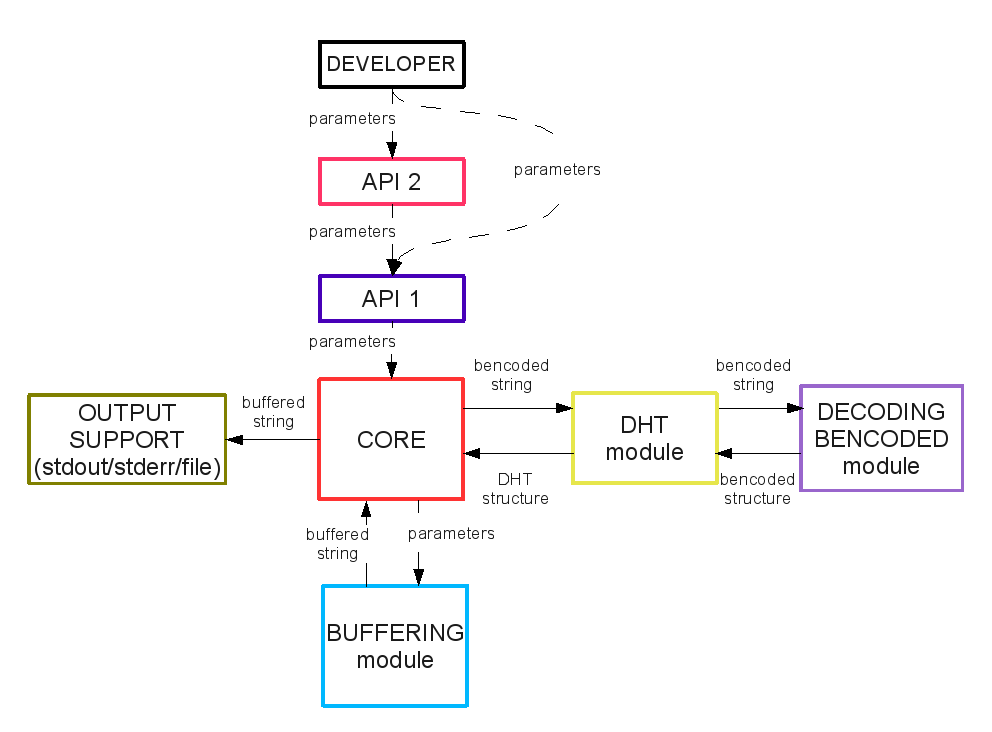
\includegraphics[scale=0.3]{img/log-library-architecture}
  \end{figure}
\end{frame}

\begin{frame}{Client Logging}
  \begin{itemize}
    \item status messages
      \begin{itemize}
        \item periodic (usually each second)
        \item client state
        \item upload speed, download speed, eta, download percentage
        \item lightweight
        \item may be monitored
      \end{itemize}
    \item verbose log messages
      \begin{itemize}
        \item per-protocol/client behavior
        \item internal events (chokes, unchokes, have, piece transmission)
        \item heavyweight
        \item cannot be monitored
        \item to be collected, parsed and disseminated
      \end{itemize}
  \end{itemize}
\end{frame}

\begin{frame}{Processing Engine}
  \begin{figure}
    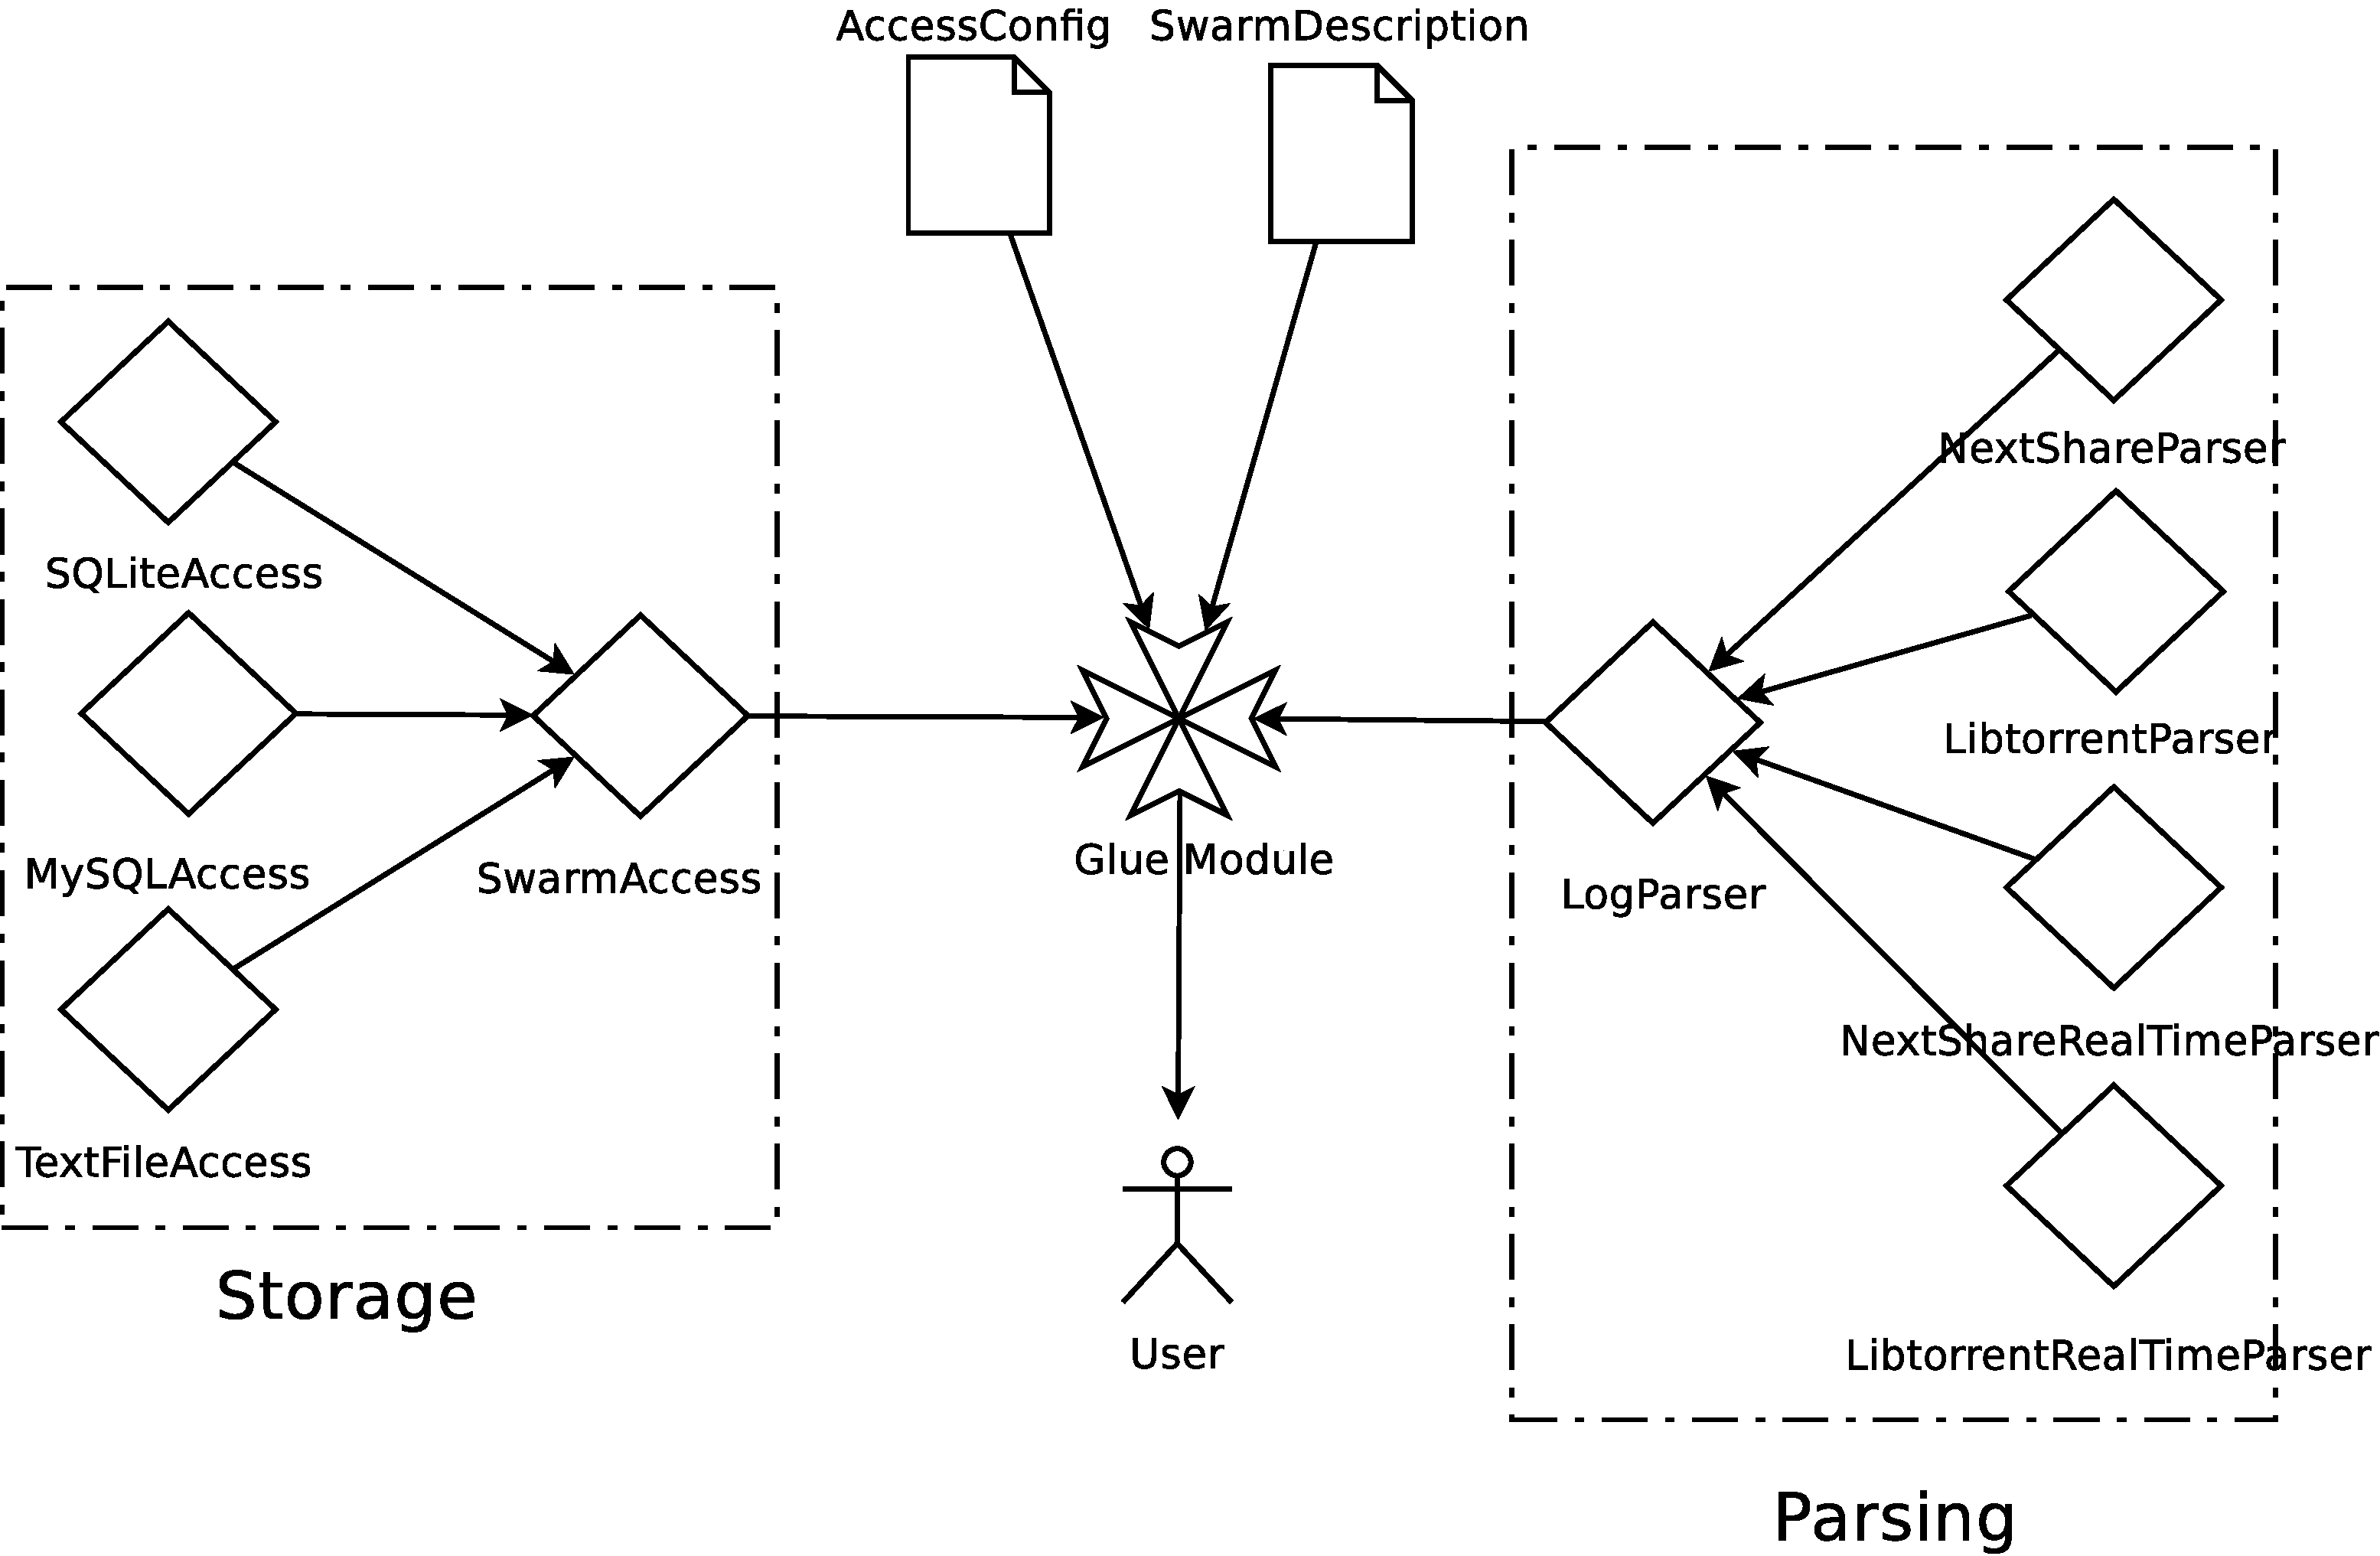
\includegraphics[scale=0.17]{img/ppf-architecture}
  \end{figure}
\end{frame}

\begin{frame}{Evaluating Performance}
  \footnotesize
  \begin{align}
    Eval(hw, sys, impl, swarm, net) = (protomsg, speed, conn, ruse)
  \end{align}
  \begin{align}
    FS = \sum_{t=0}^{DT} DS_{t}
  \end{align}
  \begin{align}
    PDS_{t} =
    \begin{pmatrix}
      ds_{1,1} = 0 & ds_{1,2} & \cdots & ds_{1,NP} \\
      ds_{2,1} & ds_{2,2} = 0 & \cdots & ds_{2,NP} \\
      \vdots & \vdots & \ddots & \vdots \\
      ds_{NP,1} & ds_{NP,2} & \cdots & ds_{NP,NP} = 0 \\
    \end{pmatrix}
  \end{align}
\end{frame}

\begin{frame}{Monitoring}
  \begin{figure}
    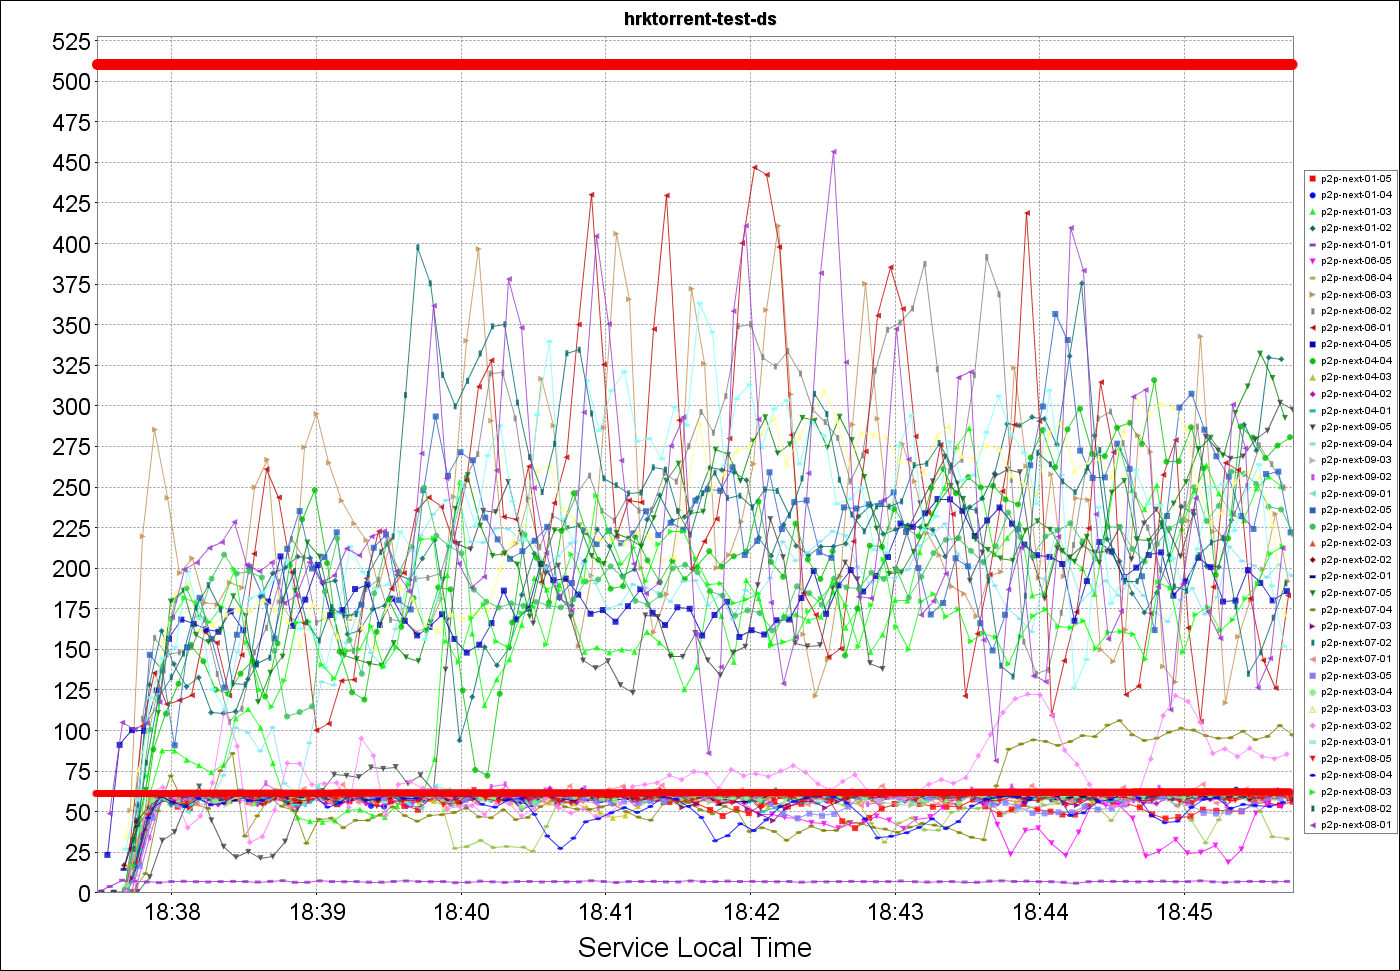
\includegraphics[scale=0.15]{img/test-monalisa-virt-env-start}
  \end{figure}
\end{frame}

\begin{frame}{Monitoring (2)}
  \begin{figure}
    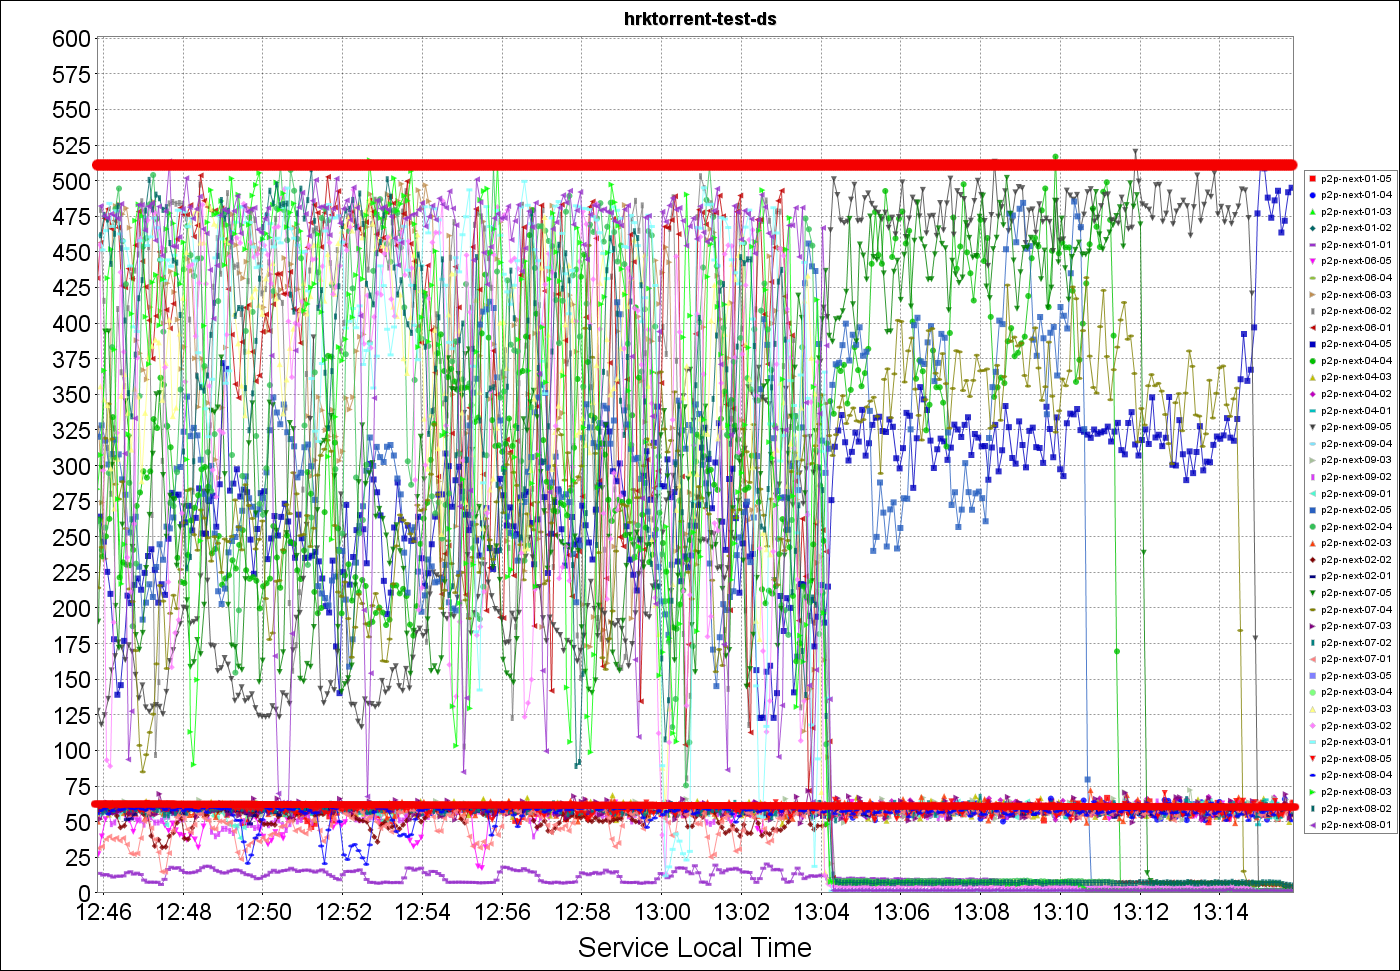
\includegraphics[scale=0.15]{img/test-monalisa-virt-env-stop}
  \end{figure}
\end{frame}

\begin{frame}{Performance Evaluation}
  \begin{table}[ht]
    \centering
    \begin{tabular}{@{}lcccc@{}}
      \toprule
      \textbf{Client} & \textbf{Test1} & \textbf{Test2} & \textbf{Test3} &
      \textbf{Test4} \\
      \midrule
      file size & 908MB & 4.1GB & 1.09GB & 1.09GB	\\
      seeders & 2900 & 761 & 521 & 496	\\
      leechers & 2700 & 117 & 49 & 51	\\
      \midrule
      aria2c & 1h17m & 53m53s & 8m & 10m23s	\\
      azureus & 32m41s & 38m33s & N/A & 7m	\\
      bittorrent & 4h53m & 60m39s & 26m & 14m	\\
      libtorrent & \textbf{9m41s} & \textbf{15m13s} & \textbf{2m30s} & \textbf{2m14s}	\\
      transmission & 40m46s & 53m & 7m & 5m	\\
      tribler & 34m & 21m & N/A & N/A		\\
      \bottomrule
    \end{tabular}
    \caption{Test Swarms Results}
    \label{table:testsw}
  \end{table}
\end{frame}

\begin{frame}{Rendering Engine}
  \begin{figure}
    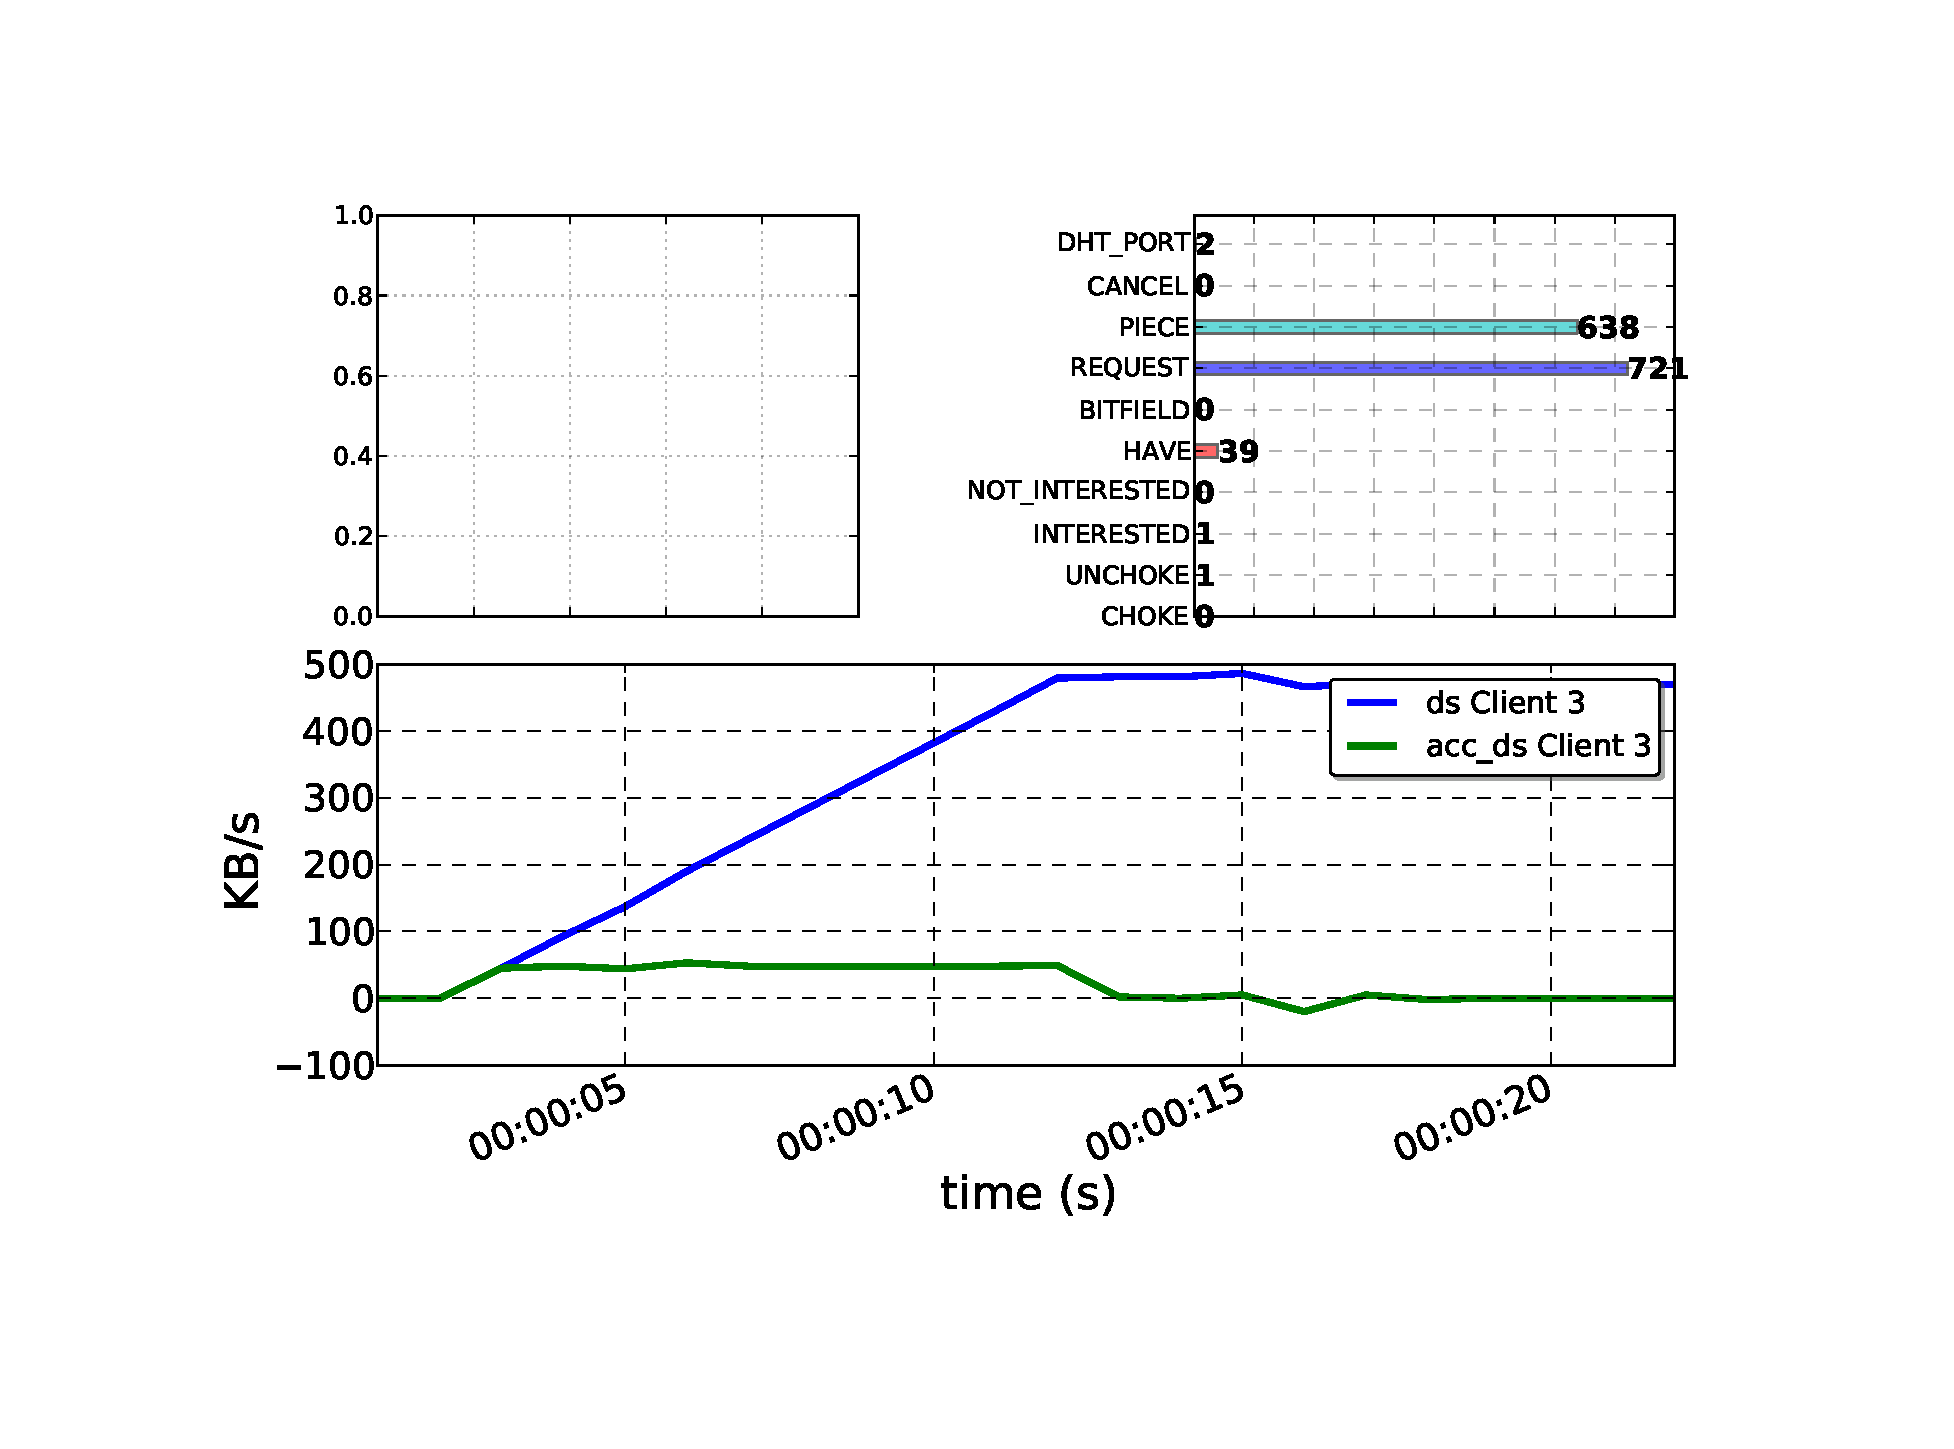
\includegraphics[scale=0.3]{img/test3}
  \end{figure}
\end{frame}

\section{Unifying BitTorrent Swarms}

\begin{frame}{Swarm Aggregation}
  \begin{itemize}
    \item different swarms sharing the same file (same info hash)
    \item clients (seeders, peers) in different swarms should see each other
    \item transparent to the client
  \end{itemize}
\end{frame}

\begin{frame}{TSUP}
  \begin{itemize}
    \item Tracker Swarm Unification Protocol
    \item UDP-based
    \item virtual connection establishment (overlay)
    \item unification
    \item updating
    \item election of a swarm leader
  \end{itemize}
\end{frame}

\begin{frame}{Sample Topology}
  \begin{figure}
    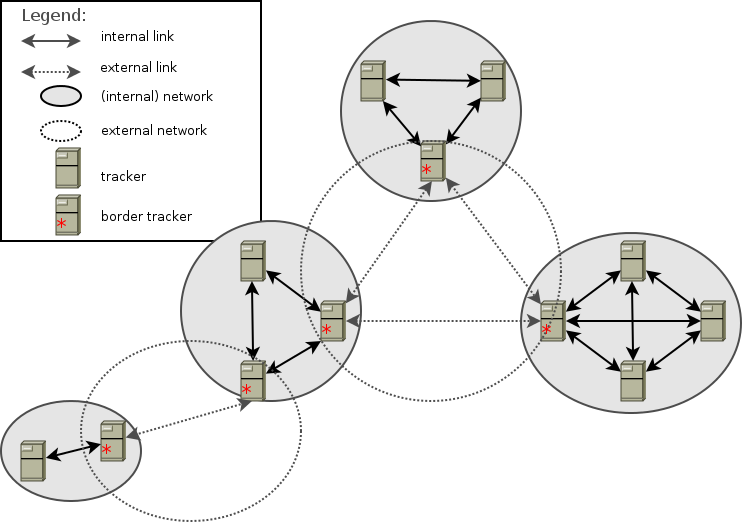
\includegraphics[width=0.8\textwidth]{img/tracker-networks.png}
  \end{figure}
\end{frame}

\begin{frame}{Message Types}
  \begin{itemize}
    \item SUMMARY: during unification, send new swarm info to a tracker
    \item UPDATE: update process
    \item HELLO: keep-alive mechanism
  \end{itemize}
\end{frame}

\begin{frame}{Keywords}
  \begin{itemize}
    \item tracker networks
    \item external link (external network, external peers)
    \item internal link (internal network, internal peers)
    \item border tracker
    \item swarm leader (internal, external) -- $O(n)$
    \item election process
  \end{itemize}
\end{frame}

\begin{frame}{Implementation}
  \begin{itemize}
    \item XBT Tracker (C++)
    \item UDP-based packets
      \begin{itemize}
        \item added \textit{UDP Tracker} in XBT
      \end{itemize}
    \item MySQL-based storage
    \item extra HTTP URIs for monitoring: \textit{trackers web page} and
    \textit{swarms web page}
  \end{itemize}
\end{frame}

\begin{frame}{Swarms/Scenarios}
  \begin{itemize}
    \item file size: 64MB, 256MB, 1024MB
    \item number of trackers: 1, 2, 4, 8, 12
    \item 4 peers per tracker (1 seeder and 3 leechers)
    \item each scenarios has been repeated 20 times
  \end{itemize}
\end{frame}

\begin{frame}{Sample Run Case}
  \begin{figure}
    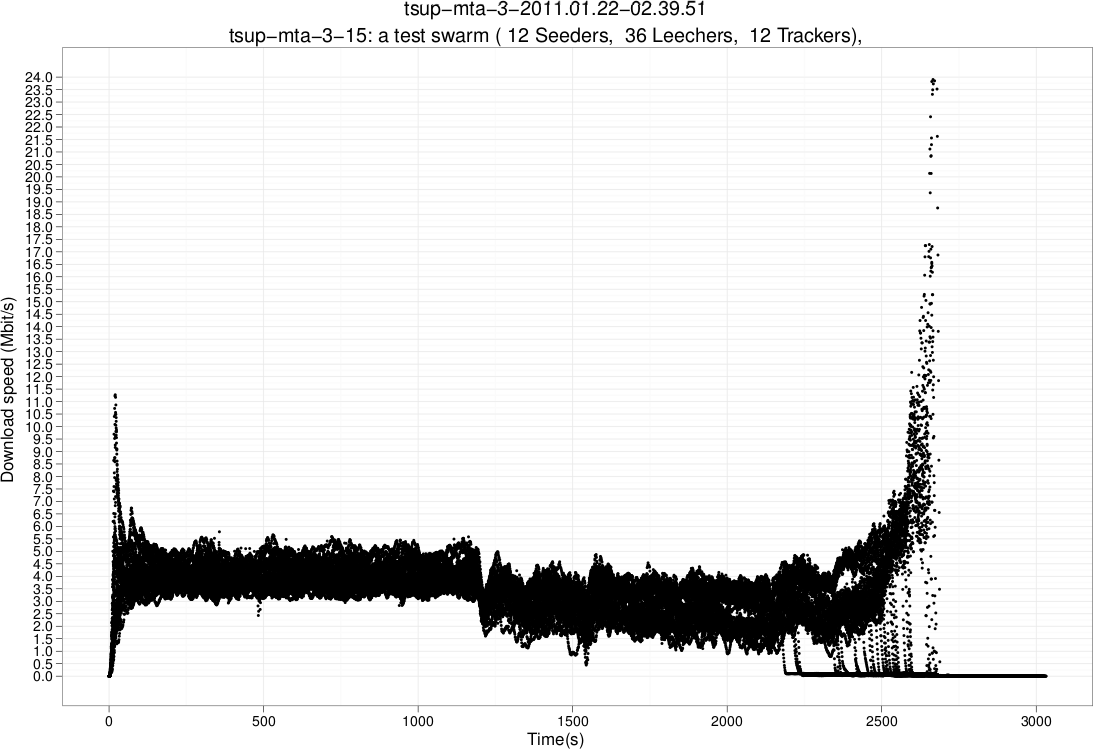
\includegraphics[width=0.8\textwidth]{img/tsup-sample-run-48peers.png}
  \end{figure}
\end{frame}

\section{Multiparty Protocol}

\begin{frame}{swift}
  \begin{itemize}
    \item radical new approach to file sharing
    \item \textit{Here is a hash! Give me data for it!}
    \item BitTorrent at Transport layer
    \item binmaps
    \item discards TCP, reliable delivery, order data
    \item current implementation on top of UDP
  \end{itemize}
\end{frame}

\begin{frame}{Multiparty Protocol}
  \begin{itemize}
    \item Transport layer implementation in the networking stack
    \item BSD socket interface
    \item issues with providing a similar interface (not-``end to end'')
  \end{itemize}
\end{frame}

\begin{frame}{Raw Socket}
  \begin{figure}
    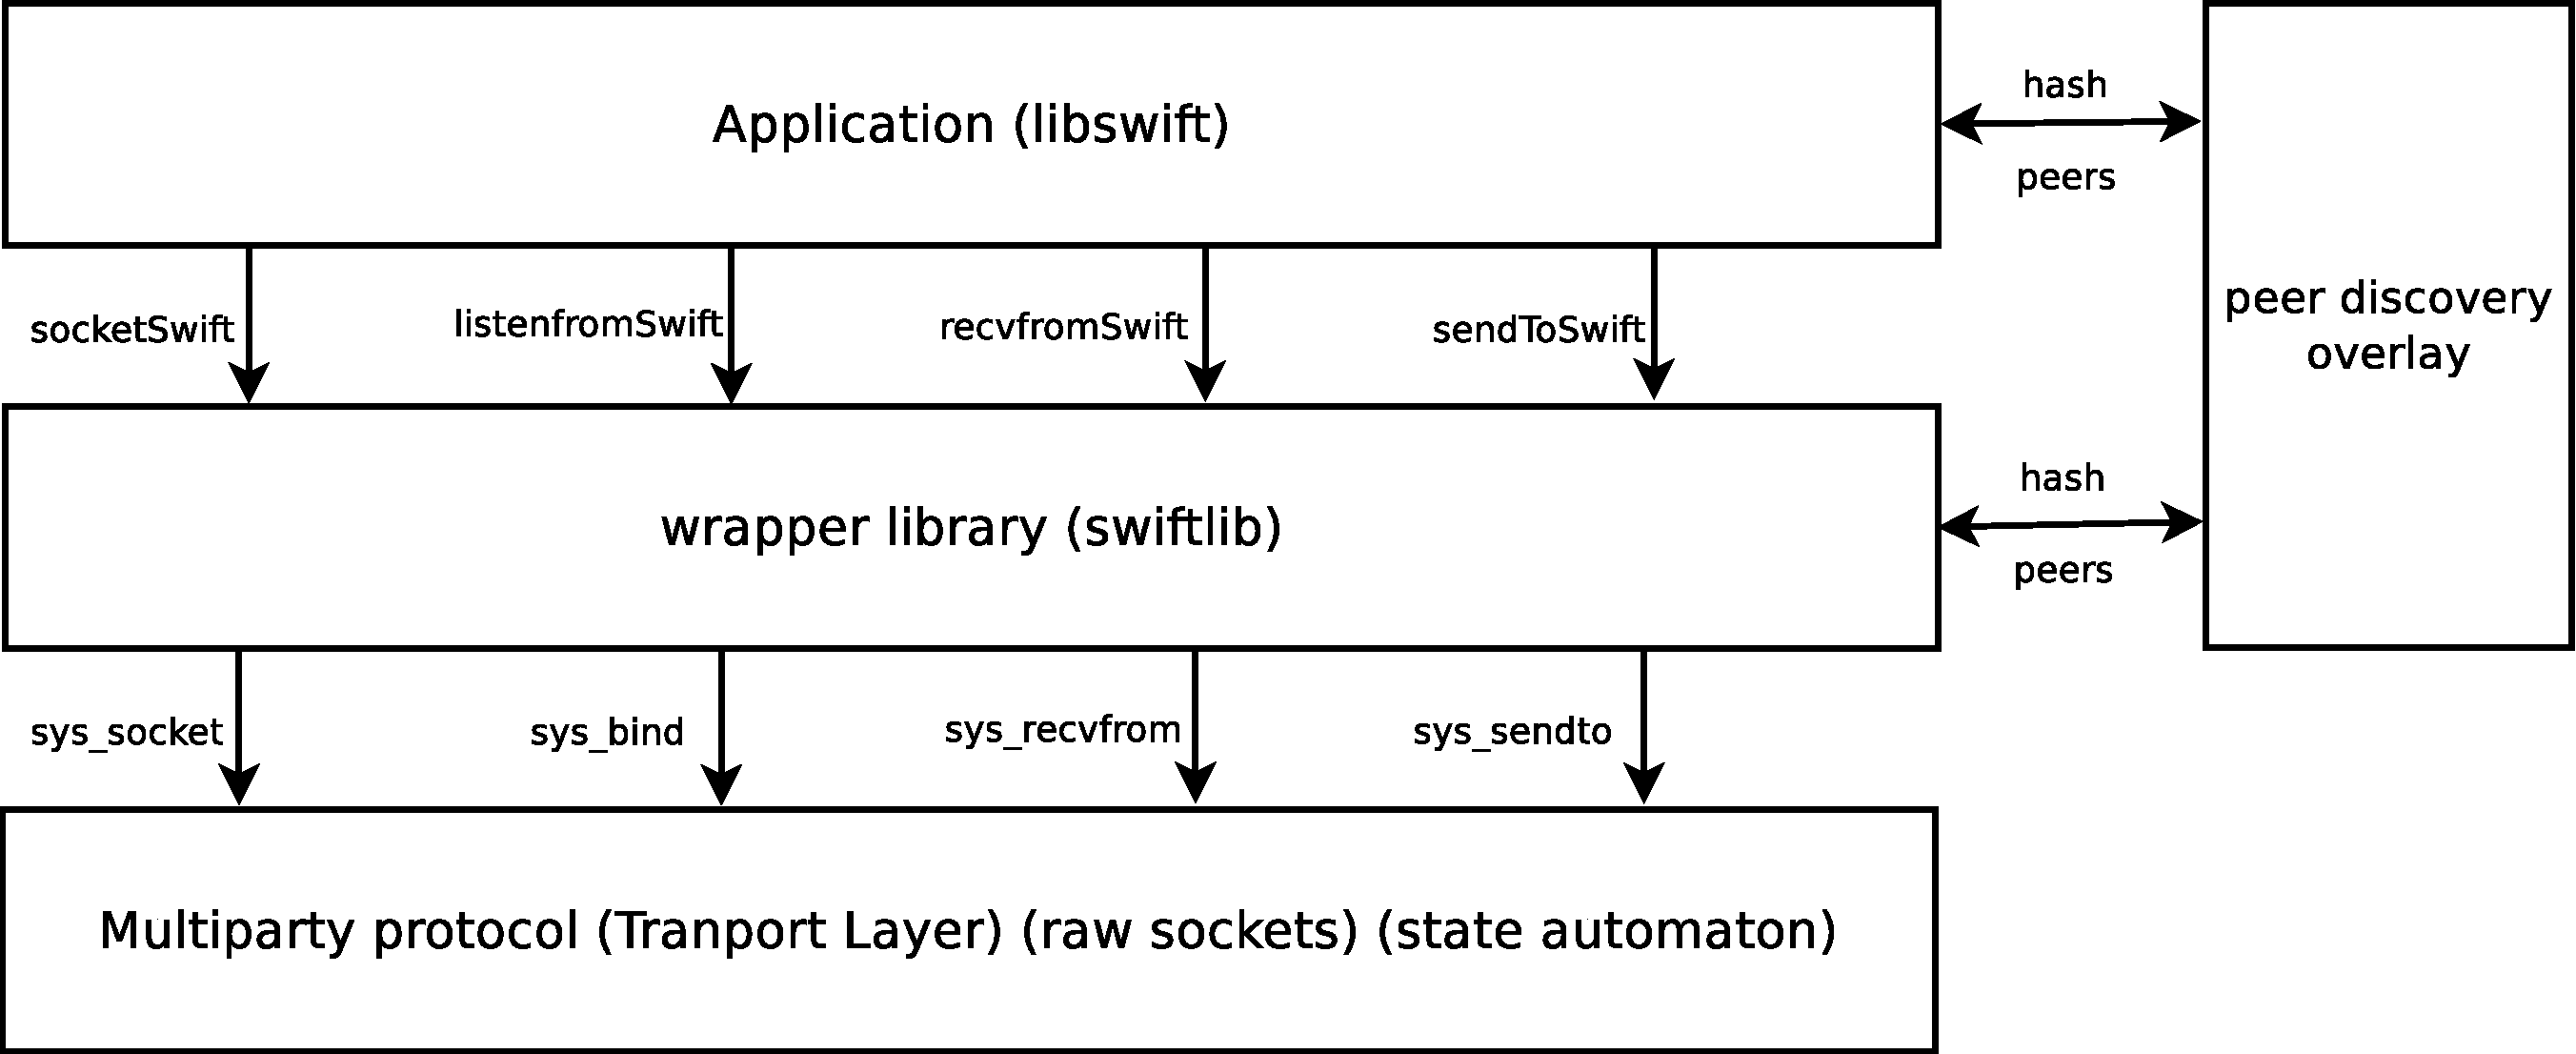
\includegraphics[width=0.8\textwidth]{img/architecture-overview}
  \end{figure}
\end{frame}

\begin{frame}{Kernel-based Approach}
  \begin{figure}
    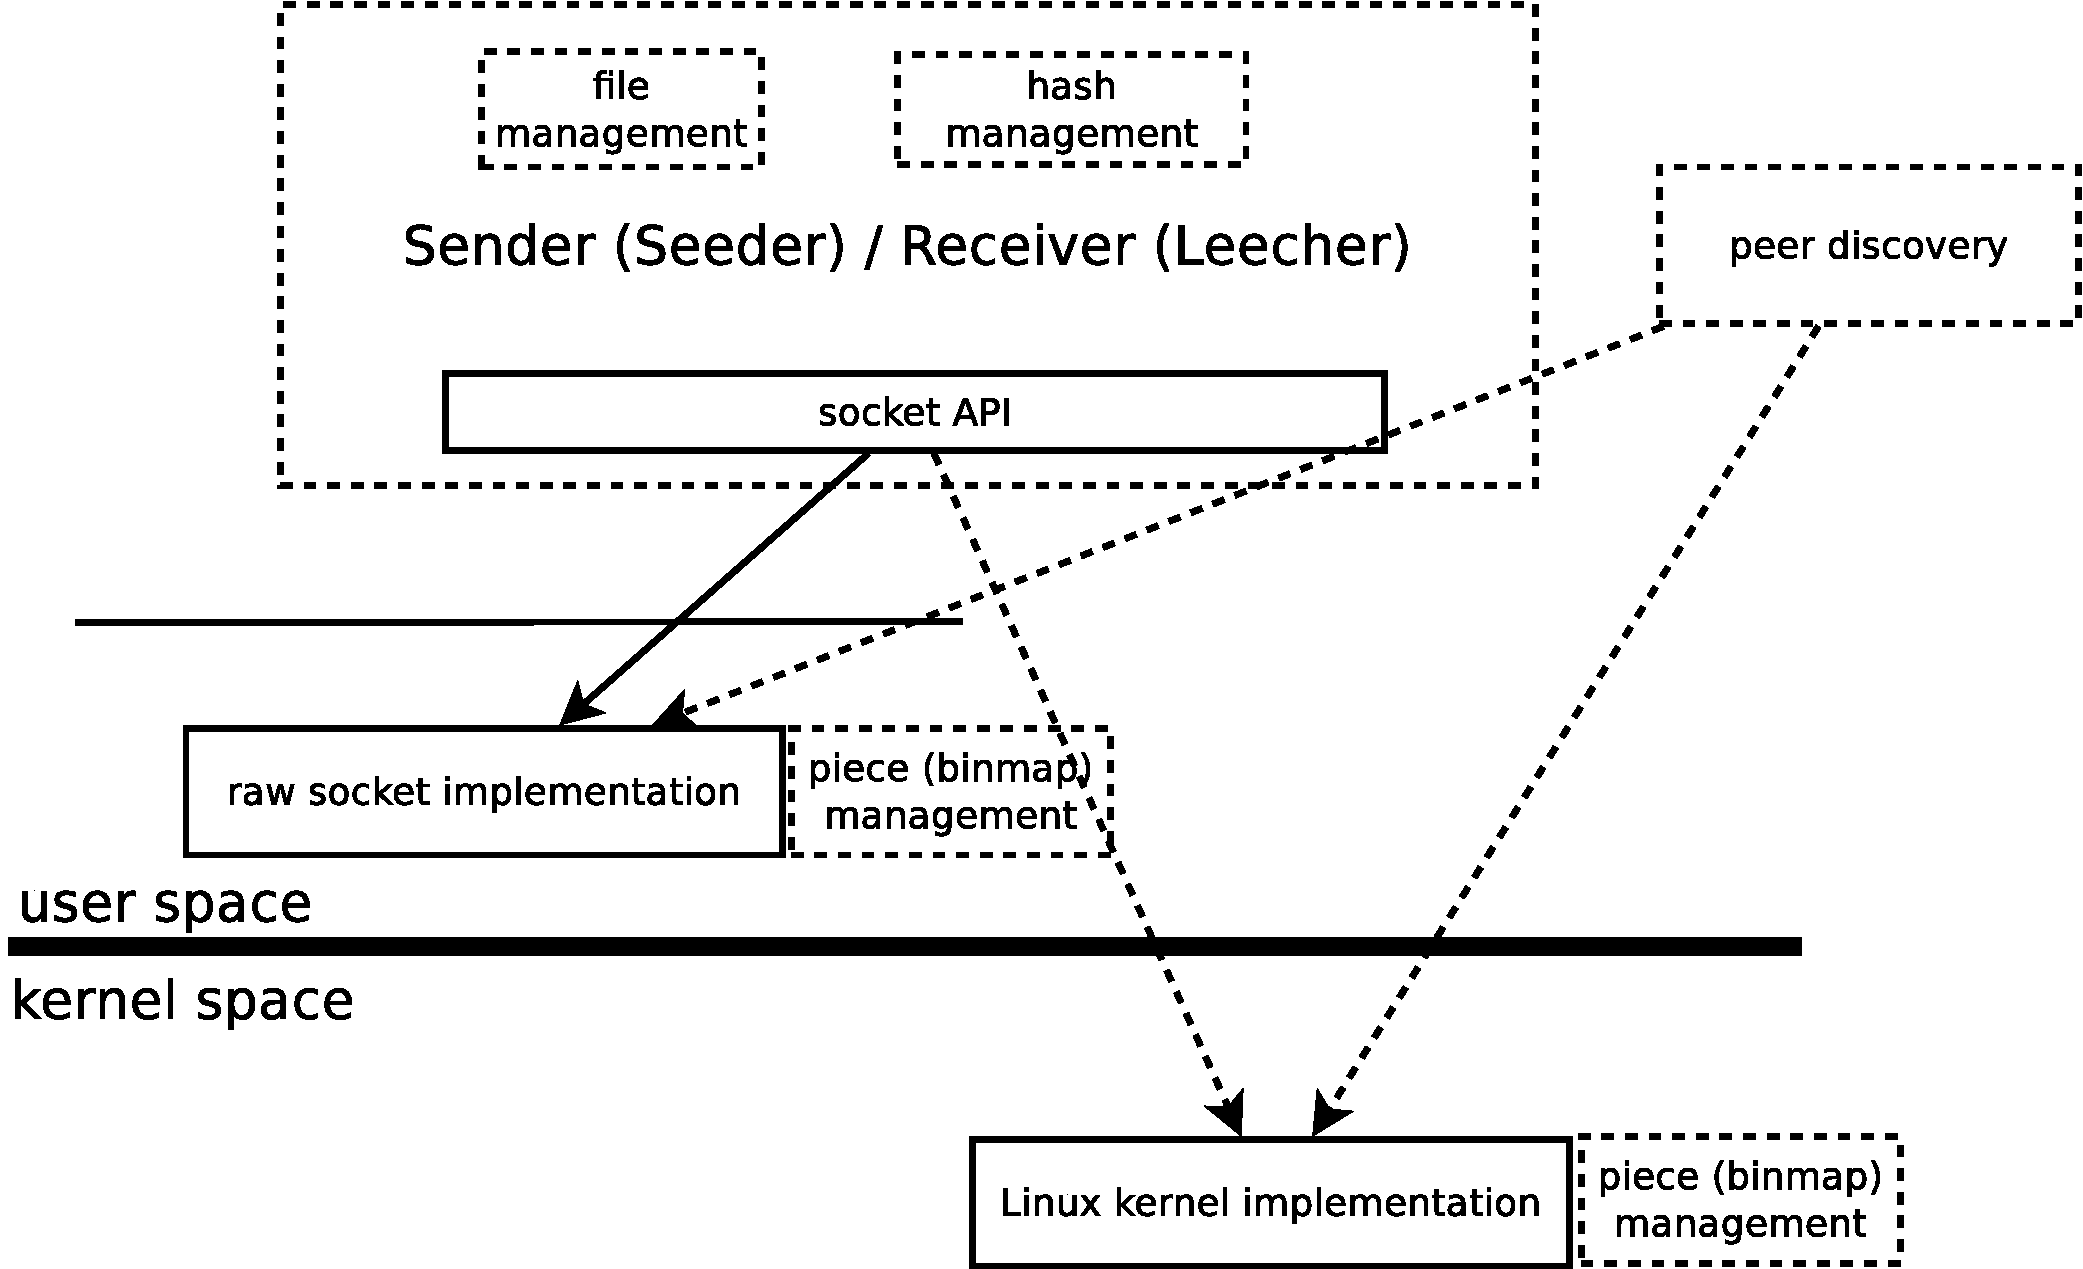
\includegraphics[width=0.8\textwidth]{img/detailed-architecture}
  \end{figure}
\end{frame}

\begin{frame}{Receiver Model}
  \begin{figure}
    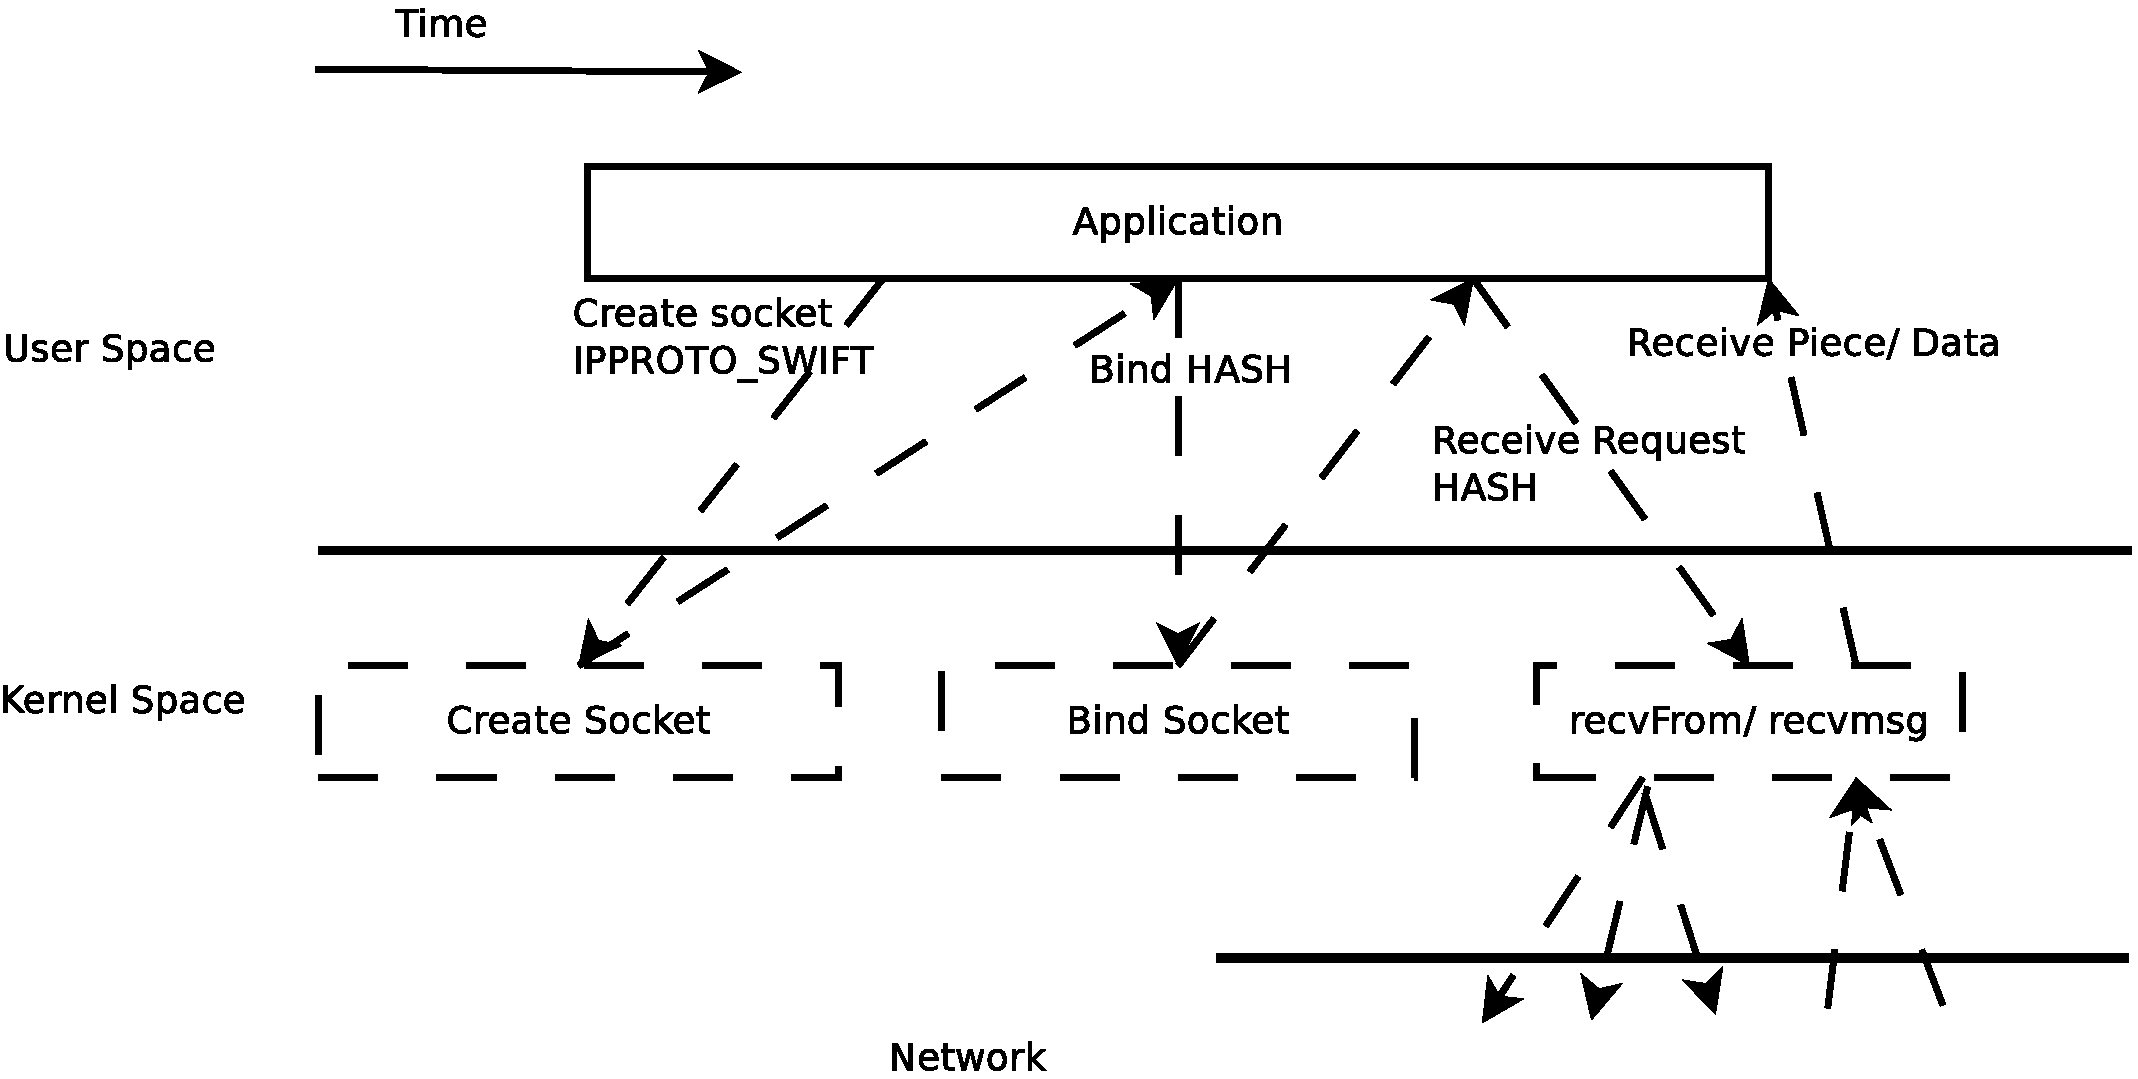
\includegraphics[width=0.9\textwidth]{img/multiparty-recvmsg}
  \end{figure}
\end{frame}

\begin{frame}{Sender Model}
  \begin{figure}
    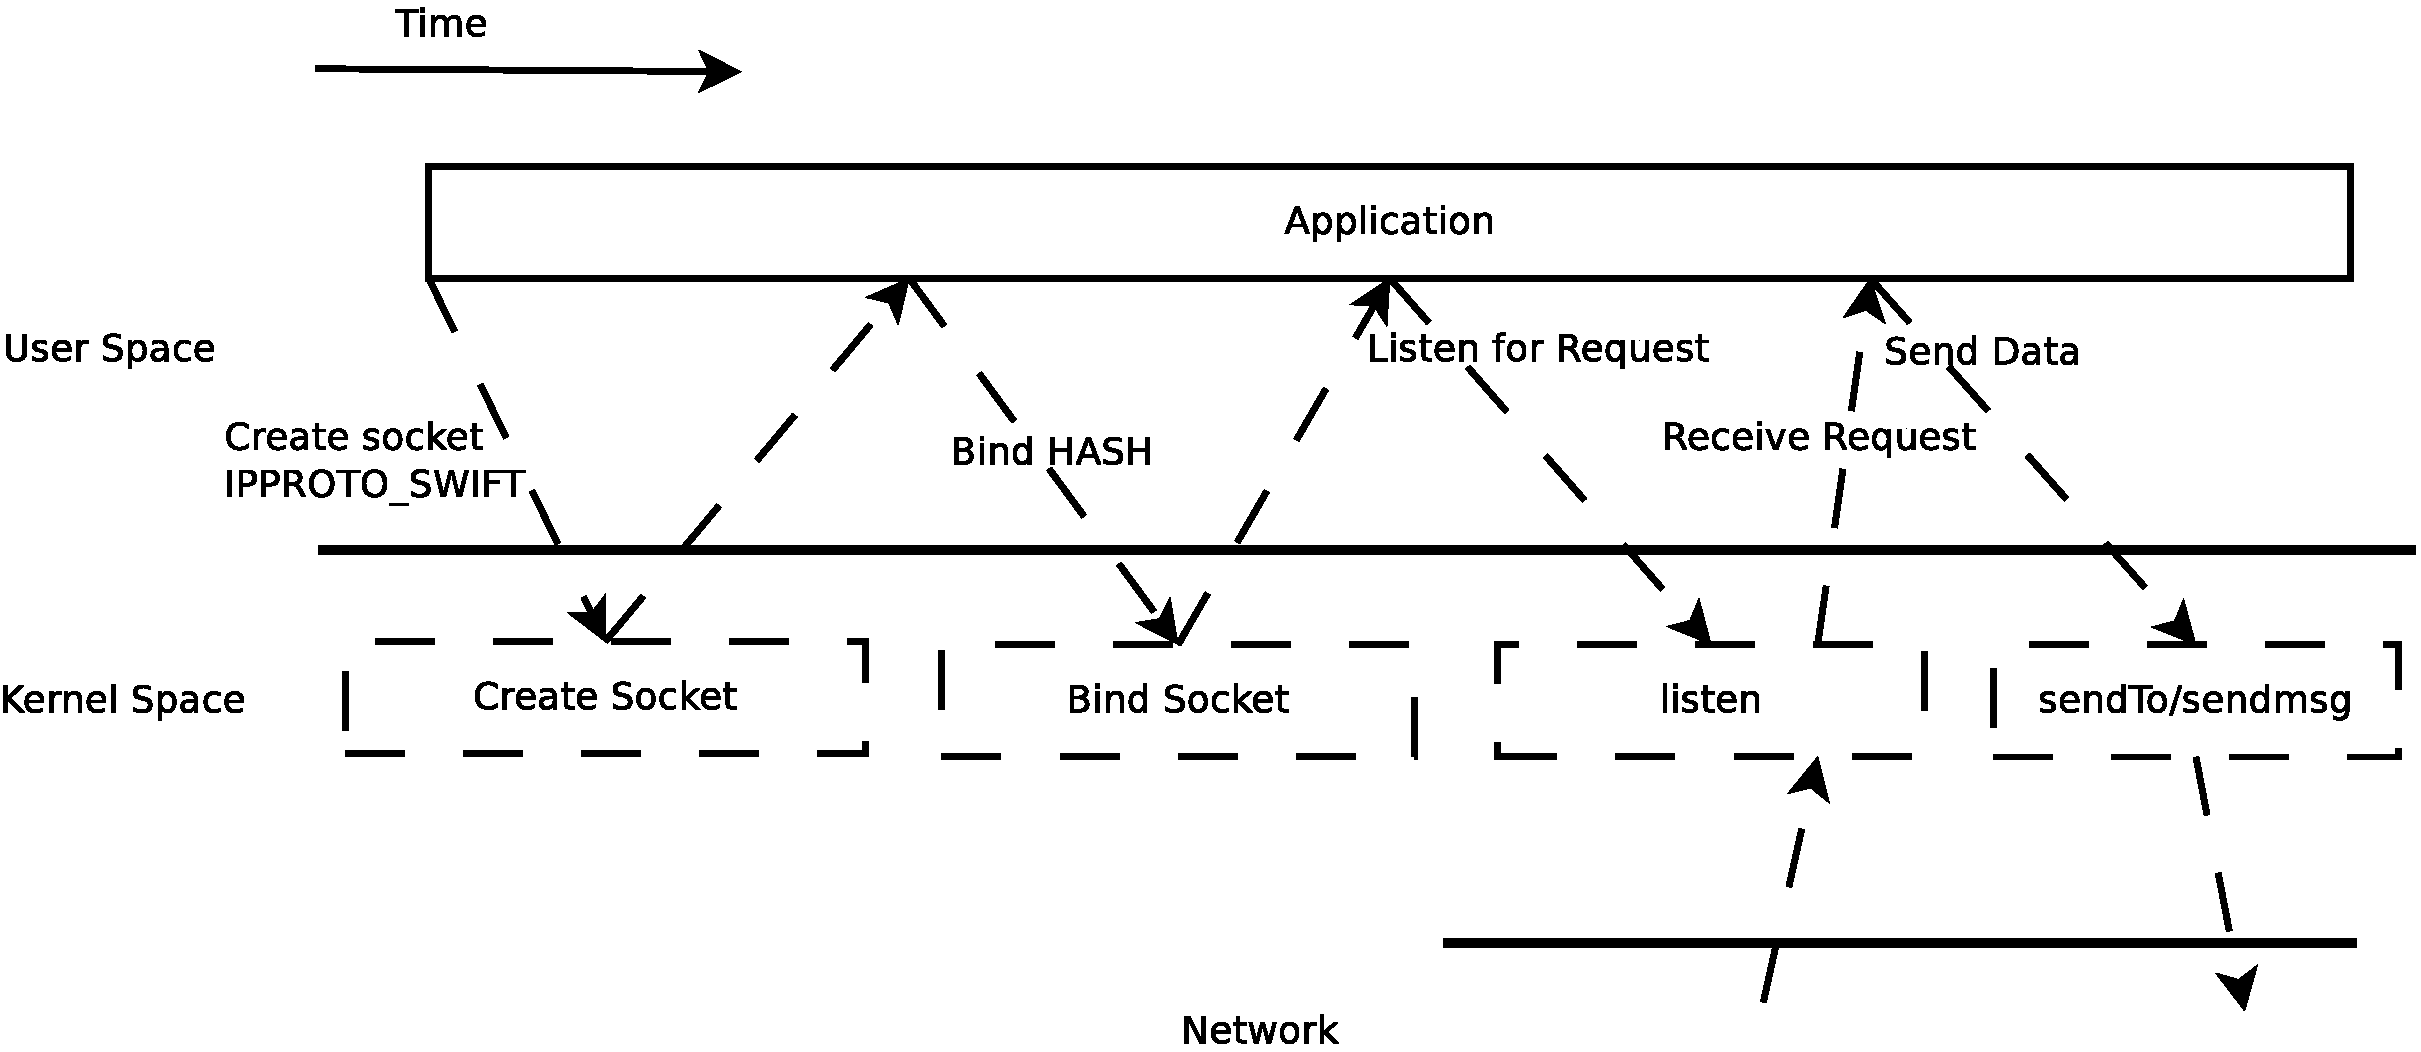
\includegraphics[width=0.9\textwidth]{img/multiparty-sendmsg}
  \end{figure}
\end{frame}

\begin{frame}{Standardization}
  \begin{itemize}
    \item current draft version
    \item talks with IEFT (PPSP group)
    \item Transport level protocol
  \end{itemize}
\end{frame}

\section{Multimedia Distribution}

\begin{frame}{Streaming Overlays in Peer-to-Peer Systems}
  \begin{itemize}
    \item update protocols to support streaming (priority on sequential
    delivery)
    \item neighbor sets
    \item peer connections $\rightarrow$ network overlay
    \item tree-based overlays
    \item mesh/swarm-based overlays
  \end{itemize}
\end{frame}

\begin{frame}{Tree-based Streaming}
  \begin{figure}
    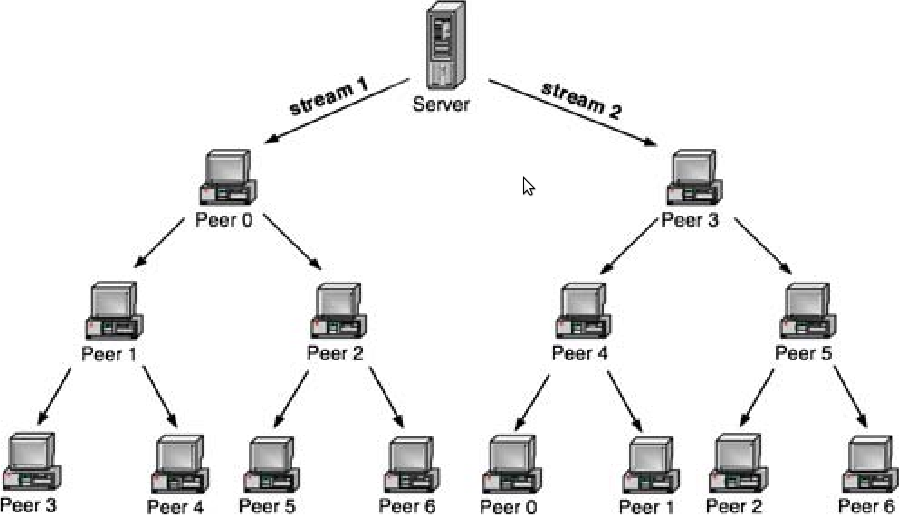
\includegraphics[width=0.9\textwidth]{img/multi-stream-tree}
  \end{figure}
\end{frame}

\begin{frame}{VoD in BiToS}
  \begin{figure}
    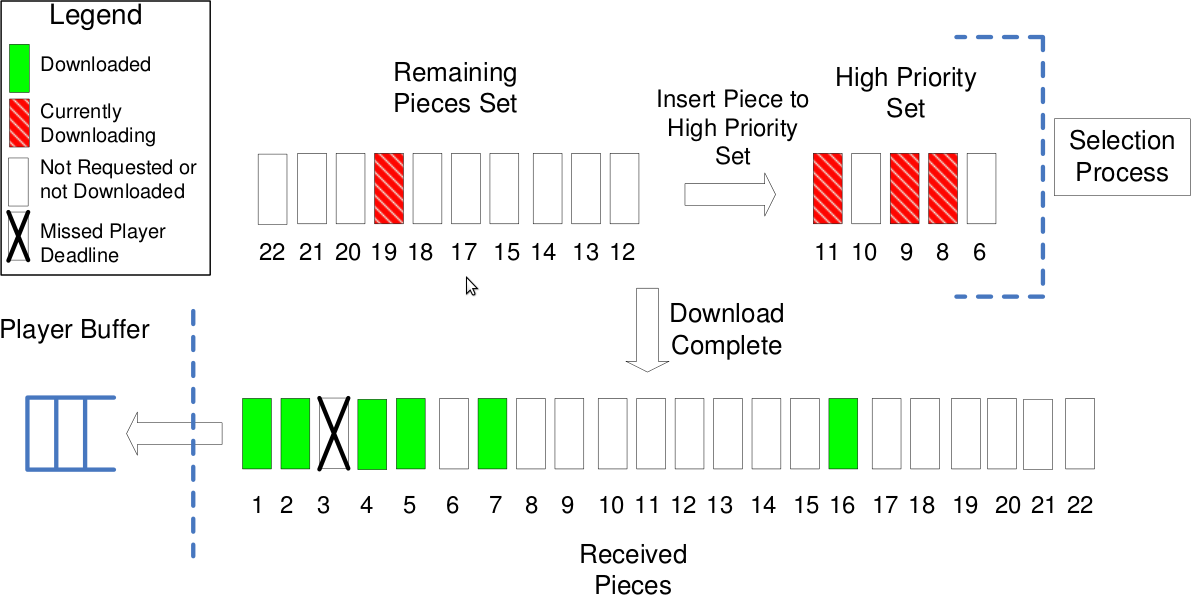
\includegraphics[width=0.9\textwidth]{img/bitos-vod}
  \end{figure}
\end{frame}

\begin{frame}{Sequential Progress}
  \begin{figure}
    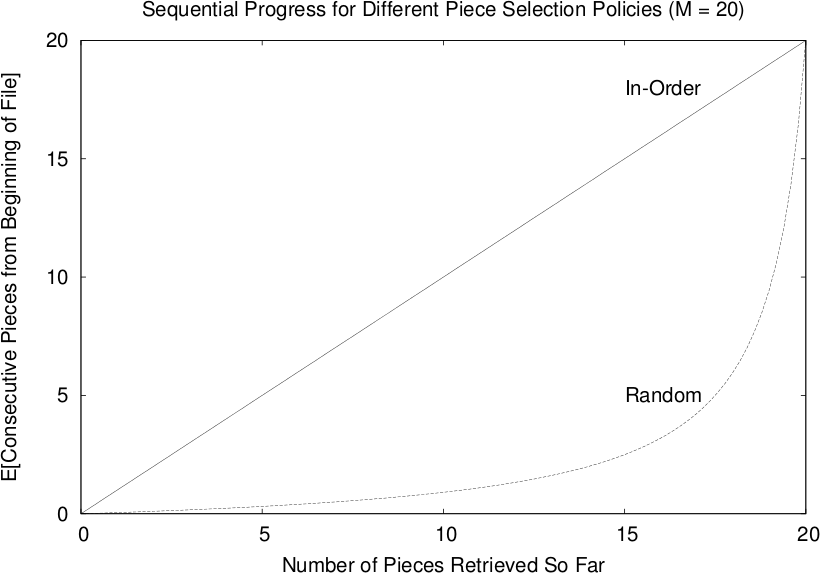
\includegraphics[width=0.9\textwidth]{img/sequential-progress}
  \end{figure}
\end{frame}

\begin{frame}{Streaming Support in libtorrent-rasterbar}
  \begin{itemize}
    \item updates to the piece picking engine
    \item \texttt{piece\_picker::pick\_pieces()}
    \item \textit{strictly in order} policy
    \item \textit{deadline-based strategy}
  \end{itemize}
\end{frame}

\begin{frame}{NextShare}
  \begin{itemize}
    \item technology, framework, core
    \item updated BitTorrent engine
    \item features such as caching, proxying, basic social networking,
    distributed search
    \item streaming support
  \end{itemize}
\end{frame}

\begin{frame}{NextSharePC}
  \begin{itemize}
    \item PC client
    \item integrated user interface
    \item standalone video player -- Swarm Player
    \item web-based browser plugin
      \begin{itemize}
        \item VLC interface (Windows, Firefox, IE)
        \item HTML5 interface (Firefox)
      \end{itemize}
  \end{itemize}
\end{frame}

\begin{frame}{LivingLab}
  \begin{itemize}
    \item infrastructure for live testing/evaluation of NextShare
    \item located in various locations of partners in P2P-Next project
    \item UPB LivingLab
    \item 10 systems from NCIT cluster
    \item site, seeders, scripts, database, log files, video files
    \item 64 GB of VoD assets
  \end{itemize}
\end{frame}

\begin{frame}{LivingLab}
  \begin{figure}
    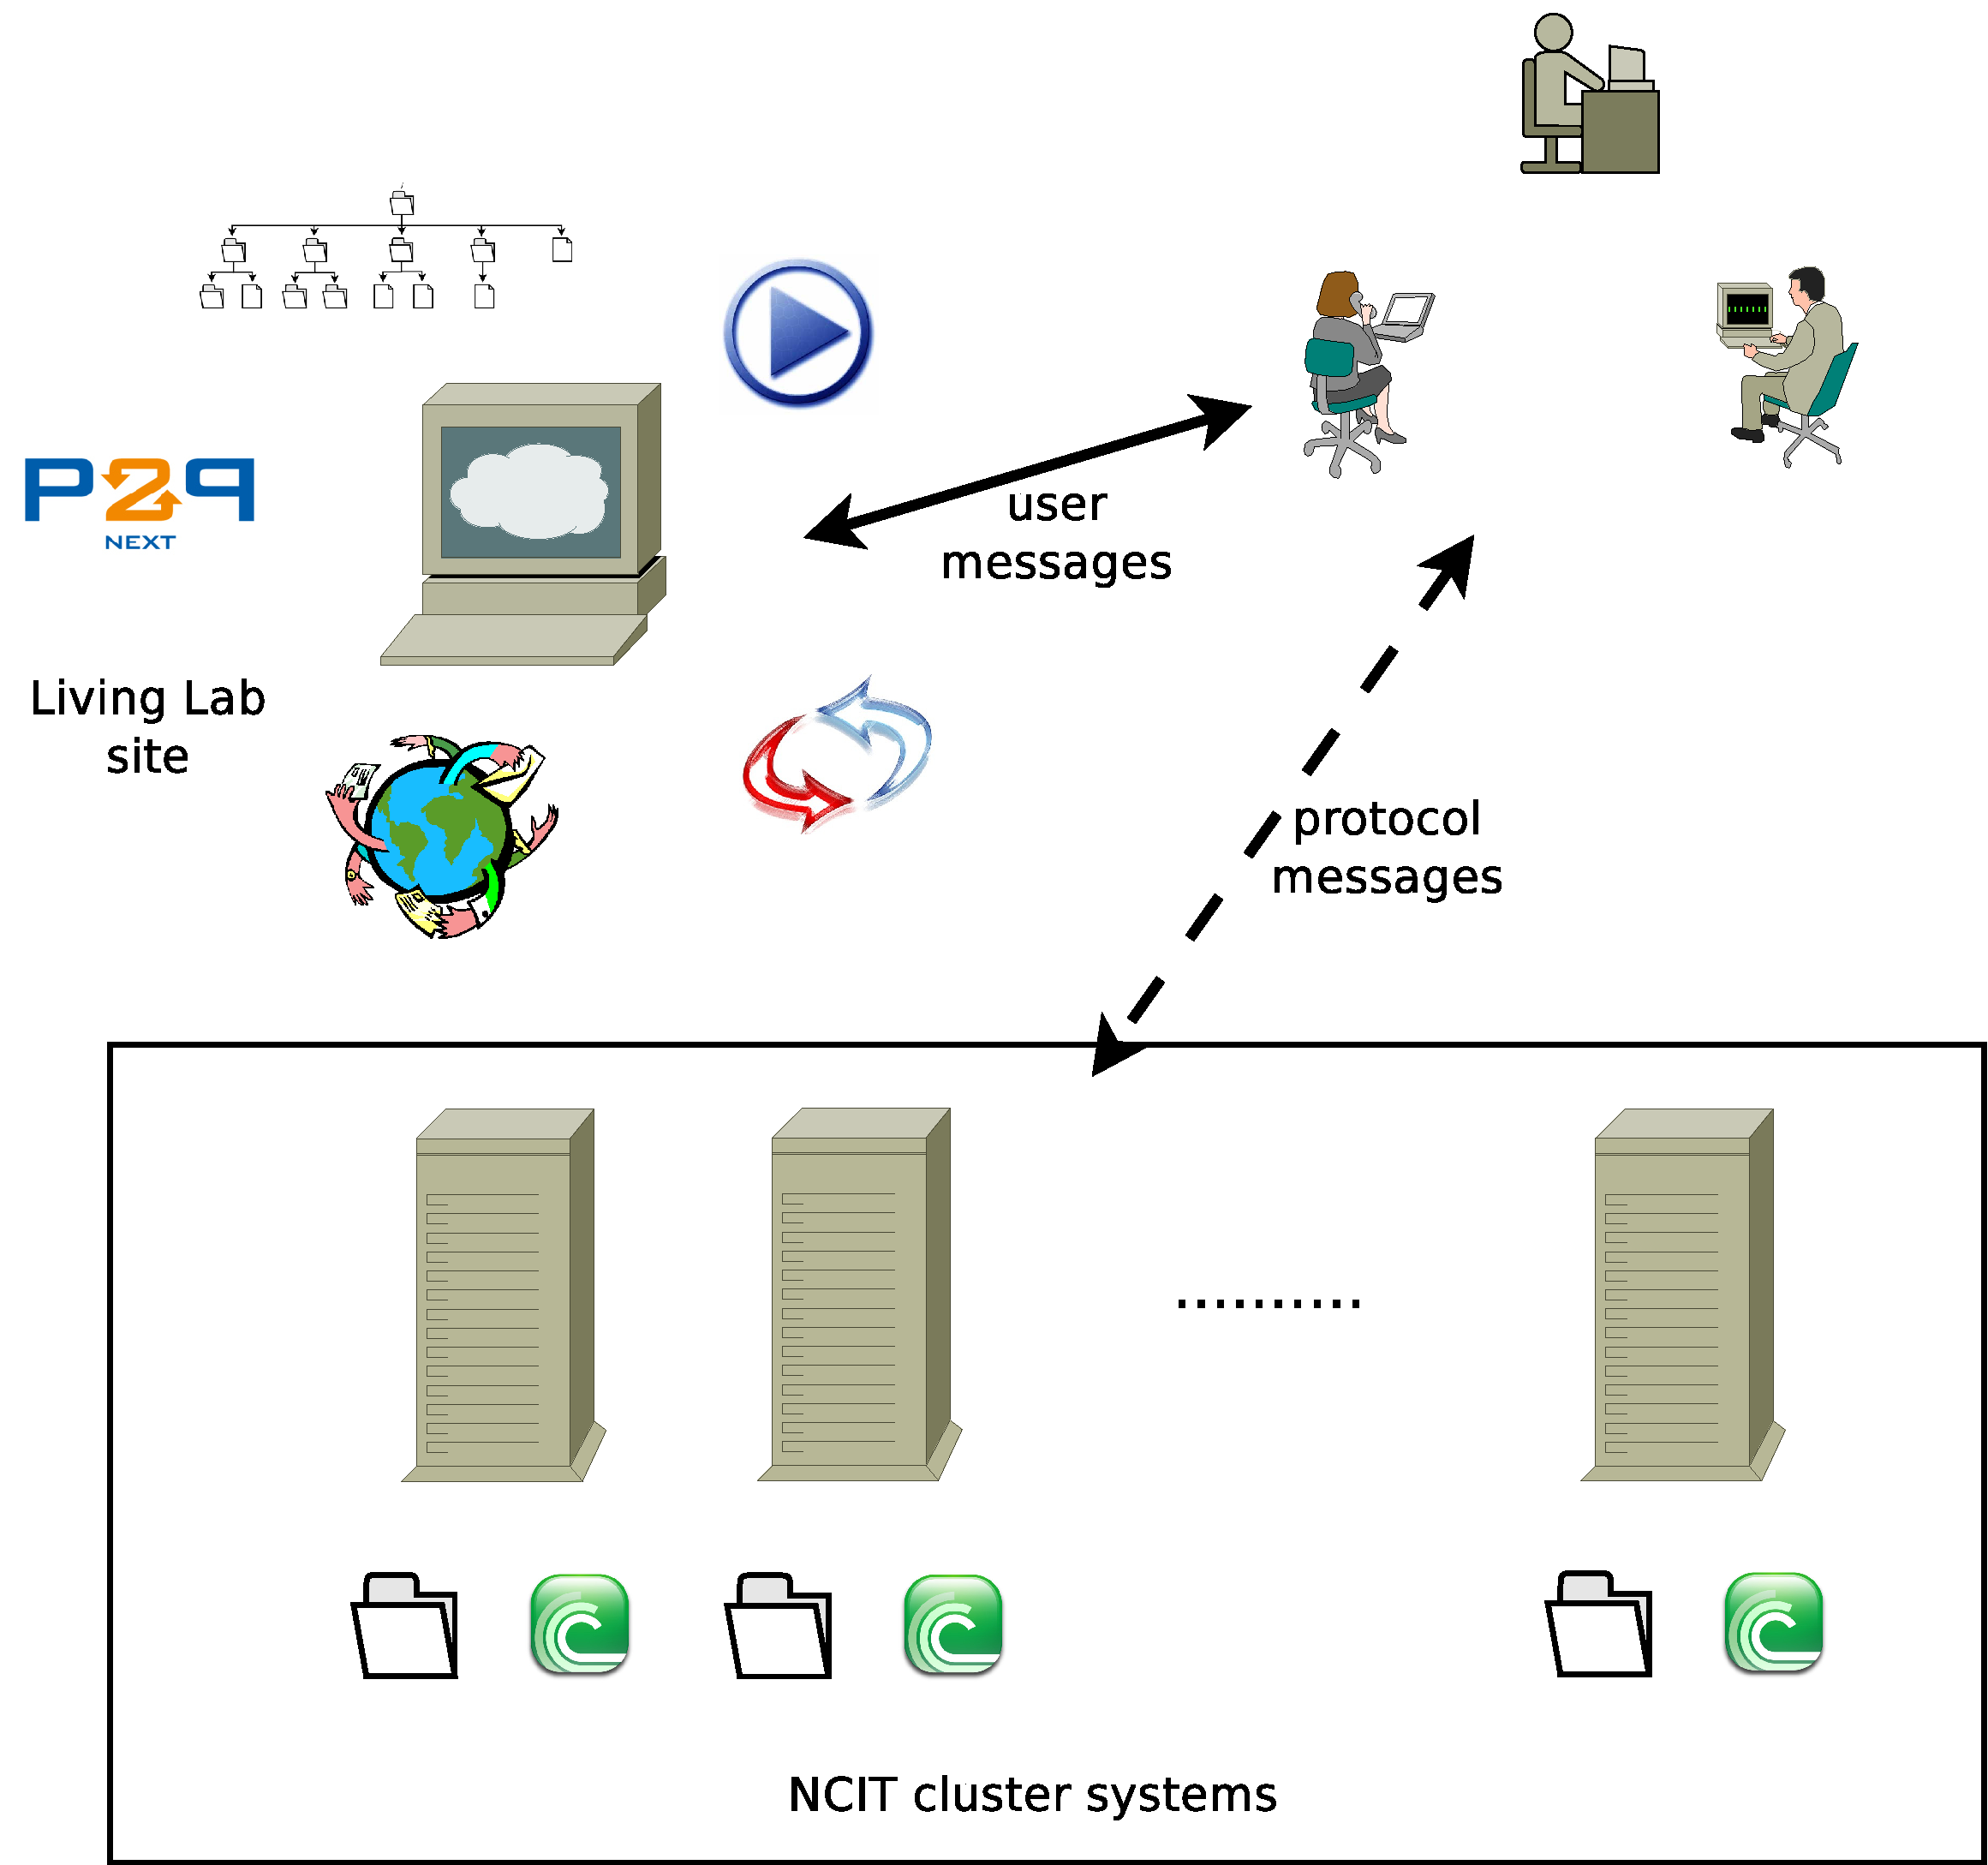
\includegraphics[width=0.6\textwidth]{img/upb-living-lab-components}
  \end{figure}
\end{frame}

\begin{frame}{LivingLab Site}
  \begin{itemize}
    \item user interface
    \item web-based NextSharePC (VLC \& HTML5)
    \item access to video files (for playback)
    \item forum
    \item feedback form
    \item an updated version under work (lightweight, user accounts, content
    ingest)
  \end{itemize}
\end{frame}

\begin{frame}{Experimental Setup}
  \begin{itemize}
    \item NCIT cluster systems
    \item seeders and tracker with logging enabled (subsequent processing)
    \item LivingLab site
    \item 64 GB of video assets
    \item support forum
    \item feedback form
    \item multiple resolutions, formats, plugins
  \end{itemize}
\end{frame}

\begin{frame}{Feedback}
  \begin{itemize}
    \item Did you have any problems during the installation?
    \item Did you successfully install the SwarmPlugin?
    \item How would you classify the quality of the video playback?
    \item How would you classify the plugin's interface?
    \item What OS are you running?
    \item What browser did you use for testing the SwarmPlugin?
    \item What was the average download speed?
  \end{itemize}
\end{frame}

\begin{frame}{Feedback Numbers}
  \begin{itemize}
    \item 55 users
    \item 42 users presented IP addresses
      \begin{itemize}
        \item 37 Romania
        \item 3 Netherlands
        \item 1 France
        \item 1 UK
      \end{itemize}
    \item video playback classification: 2.41
    \item plugin interface classification: 3.02
    \item IE: 10, Firefox: 28, Dual: 17
  \end{itemize}
\end{frame}

\begin{frame}{Feedback Results}
  \begin{itemize}
    \item lack of plugin on several platforms
    \item playback problems
    \item no video handling buttons
    \item content delivery
    \item long buffering
    \item installer updates
    \item dual functionality (installer should work on IE \textbf{and} Firefox)
  \end{itemize}
\end{frame}

\begin{frame}{Results}
  \begin{figure}
    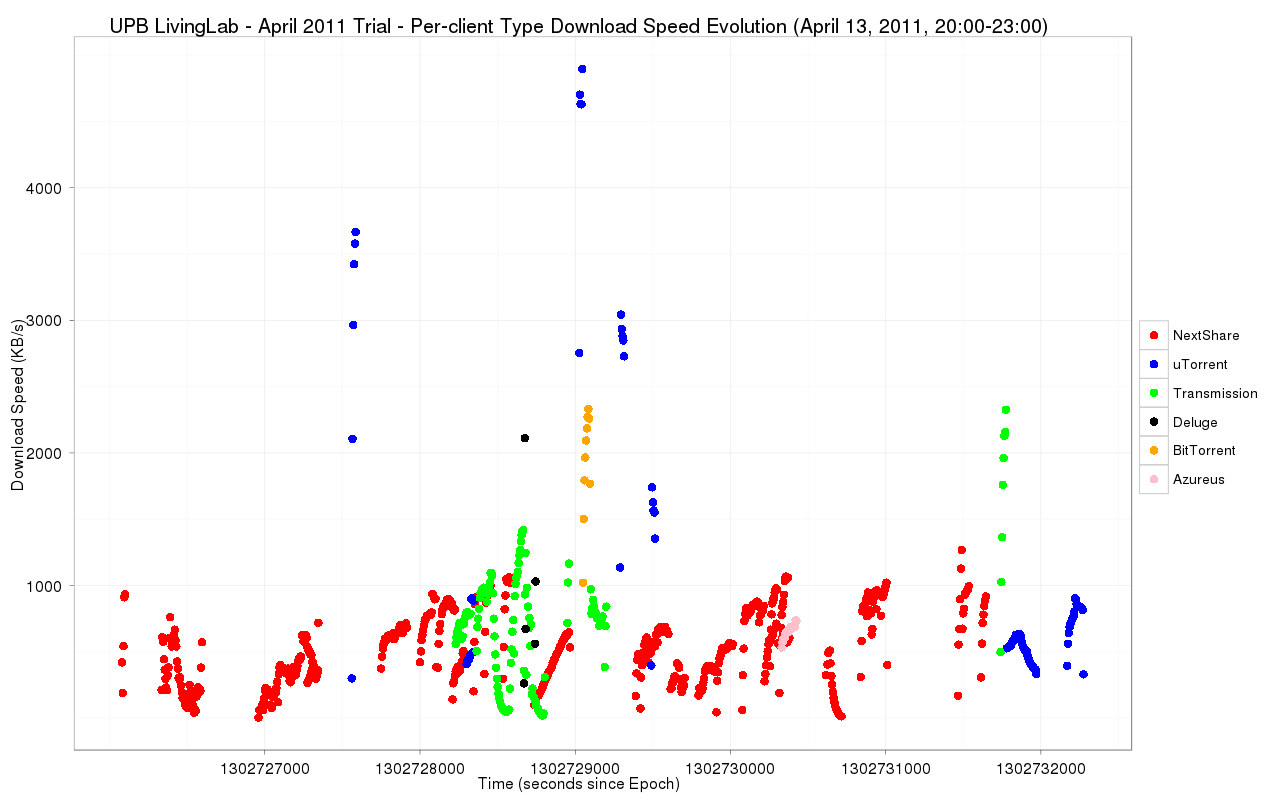
\includegraphics[width=0.8\textwidth]{img/ll-trial}
  \end{figure}
\end{frame}

\section{Conclusion}

\begin{frame}{Contributions}
  \begin{itemize}
    \item fully automated and scalable infrastructure
    \item virtualization technology in the context of Peer-to-Peer systems
    \item simulating connection dropouts in BitTorrent environments
    \item updates and patches to existing BitTorrent
    \item classification of protocol messages types and protocol parameters
    \item generic logging library
    \item a protocol parameter parsing and analysis engine
    \item streaming support to the popular libtorrent implementation
    \item deployment and maintenance of the local Living Lab
    \item analysis and monitoring of BitTorrent streaming
    \item swarm unification tracker overlay
    \item integration the kernel space as a multiparty transport protocol
  \end{itemize}
\end{frame}

\begin{frame}{Further Work}
  \begin{itemize}
    \item complete multiparty protocol implementation
    \item standardization of multiparty protocol
    \item enhance virtualized infrastructure
    \item fill model for virtualization adequacy
    \item verify formal evaluation of Peer-to-Peer parameters
    \item classical distribution versus streaming
  \end{itemize}
\end{frame}

\begin{frame}{Talks}
  \begin{itemize}
    \item Performance of P2P Implementations. P2P'08 Workshop. Aachen, September
    2008
    \item Peer-to-Peer Systems. Evolution and Challenges. Ixia HiTech
    Presentations. Bucharest, April 2011
  \end{itemize}
\end{frame}

\begin{frame}{Papers}
  \begin{itemize}
    \scriptsize
    \item Mircea Bardac, George Milescu, and Răzvan Deaconescu. Monitoring a
    BitTorrent Tracker for Peer-to-Peer System Analysis. In \textit{Intelligent
    Distributed Computing}, pages 203--208, 2009
    \item Călin-Andrei Burloiu, Răzvan Deaconescu, and Nicolae Țăpuș. Design and
    Implementation of a BitTorrent Tracker Overlay for Swarm Unification. In
    \textit{International Conference on Network Services}, 2011
    \item Răzvan Deaconescu, George Milescu, Bogdan Aurelian, Răzvan Rughiniș,
    and Nicolae Țăpuș. A Virtualized Infrastructure for Automated BitTorrent
    Performance Testing and Evaluation. \textit{International Journal on
    Advances in Systems and Measurements}, 2(2\&3):236--247, 2009
    \item Răzvan Deaconescu, George Milescu, and Nicolae Țăpuș. Simulating
    Connection Dropouts in BitTorrent Environments. In \textit{EUROCON --
    International Conference on Computer as a Tool}, 2011, IEEE, pages 1-4, 2011
    \item Răzvan Deaconescu, Răzvan Rughiniș, and Nicolae Țăpuș. A BitTorrent
    Performance Evaluation Framework. \textit{Proceedings of Fifth International
    Conference of Networking and Services}, 2009
    \item Răzvan Deaconescu, Răzvan Rughiniș, and Nicolae Țăpuș. A Virtualized
    Testing Environment for BitTorrent Applications. \textit{Proceedings of
    CSCS'17}, 2009
  \end{itemize}
\end{frame}

\begin{frame}{Papers (2)}
  \begin{itemize}
    \scriptsize
    \item Răzvan Deaconescu, Marius Sandu-Popa, Adriana Drăghici, and Nicolae
    Țăpuș. Using Enhanced Logging for BitTorrent Swarm Analysis. In
    \textit{Proceedings of the 9th RoEduNet IEEE International Conference},
    Sibiu, 2010
    \item Răzvan Deaconescu, Marius Sandu-Popa, Adriana Drăghici, and Nicolae
    Țăpuș. BitTorrent Swarm Analysis through Automation and Enhanced Logging.
    \textit{International Journal of Computer Networks \& Communications},
    3(1):53--65, 2011
    \item Andreea Leța, Răzvan Deaconescu and Răzvan Rughiniș. Extending Packet
    Altering Capacities in Simulated Large Networks. In \textit{Proceedings of
    the 17th International Conference on Control Systems and Computer Science
    (CSCS17)}, Bucharest, 2009
    \item Marius Sandu-Popa, Adriana Drăghici, Răzvan Deaconescu, and Nicolae
    Țăpuș. A Peer-to-Peer Swarm Creation and Management Framewor. In
    \textit{Proceedings of the 1st Workshop on Software Services: Frameworks and
    Platforms}, Timișoara, Romania, 2010
    \item George Milescu, Răzvan Deaconescu, and Nicolae Țăpuș. Versatile
    Configuration and Deployment of Realistic Peer-to-Peer Scenarios. In
    \textit{International Conference on Network Services}, 2011
  \end{itemize}
\end{frame}

\section{Questions}

\end{document}
